\Chapter{PLONGEMENTS VECTORIELS DE GRAPHES DE CONNAISSANCES}
\label{chap:kge}

Ce chapitre introduit les modèles de plongement vectoriels, utilisés pour représenter les entités et les relations d'un graphe de connaissance sous forme vectorielle. Ces représentations vectorielles, dont la géométrie intègre une partie de l'information sémantique contenue dans le graphe, permettent l'application d'outils d'apprentissage automatique, comme la complétion de triplets \cite{simple2018}, la détection de triplets invalides \cite{nguyen2020relational}, mais aussi l'extraction automatique de taxonomie qui fait l'objet de ce mémoire \cite{ristoski2017large, zhang2018taxogen}. Dans ce chapitre, on présente dans le détail les modèles utilisés dans la suite de notre travail, en distinguant deux façons d'envisager les modèles de plongement – l'une géométrique, l'autre algébrique. On s'attache notamment à mettre en évidence les hypothèses de chaque modèle, les types de relations qu'il s'attache à modéliser, et les implications des choix effectués pour la modélisation. % Au-delà des deux familles de modèles présentées, on propose également un survol des autres approches existantes dans la littérature.

Enfin, on présente une nouvelle tâche sur laquelle évaluer un modèle de plongement de graphe. Cette tâche vise explicitement à mesurer la capacité d'un modèle à envoyer des entités appartenant à une même classe dans une même région de l'espace – une propriété essentielle pour pouvoir extraire des informations taxonomiques à partir des plongements vectoriels, et un préalable aux méthodes présentées dans les chapitres suivants de ce mémoire.


\section{Généralités}
\label{sec:kge-general}


\subsection{Introduction et motivation}
\label{subsec:kge-general-intro}



Dans toute cette section, on considérera un graphe de connaissance $\KG \subseteq \Ent \times \Rel \times \Ent$ dont on notera $n = | \Ent |$ le nombre d'entités, et $m = |\Rel |$ le nombre de relations.

% \todo{Reformuler, en partant des différents modes de représentation}

\subsubsection{Représentation des entités et des relations d'un graphe}
\newcommand{\IRI}{\operatorname{IRI}}
\newcommand{\Adja}{\operatorname{Adj}}

La représentation des données est une question cruciale en apprentissage automatique; or la représentation standard des entités dans un graphe de connaissance est très inadaptée à la plupart des algorithmes. En effet, dans un graphe de connaissance RDF, une ressource est représentée par un identifiant unique, l'IRI (\textit{International Resource Identifier}). 
Une IRI est purement symbolique et ne contient pas nécessairement d'information sur la ressource qu'elle représente. %  ou peu d'information sur la ressource qu'elle représente.
Cette représentation discrète ne permet pas, par exemple, de comparer deux entités entre elles : pour deux entités $e$ et $e'$, la seule donnée de leurs IRI respectives ne permet pas de déduire si ces entités sont proches l'une de l'autre. %Cela n'est pas un problème pour un système logique basé sur des axiomes et des règles d'inférences; pour un algorithme d'apprentissage automatique 
% si deux entités $e$ et $e'$ sont représentées par leurs IRI $\IRI(e)$ et $\IRI(e')$, on peut savoir que $e = e'$ si $r=r'$; dans le cas $r \neq r'$, on ne peut rien conclure. 

Certains auteurs combinent IRI et plongements lexicaux pour obtenir des représentations vectorielles des entités d'un graphe \cite{socher2013reasoning}. Pour cela, on découpe l'IRI (ou éventuellement le nom de l'entité, tel qu'indiqué par la relation \texttt{rdfs:label}) en mots, on récupère les plongements lexicaux de ces mots (c'est-à-dire des représentations vectorielles de mots en faible dimension, comme par exemple Word2Vec \cite{mikolov2013distributed}), et on combine ces plongements, par exemple en les moyennant.
Une telle représentation permet alors de mesurer une distance entre entités, et permet l'application d'algorithmes d'apprentissage automatique. Elle présente toutefois un inconvénient sévère : les plongements lexicaux sont appris sur des corpus textuels génériques et extérieurs au graphe. En ce sens, ces plongements échouent à représenter le contenu et les propriétés intrinsèques du graphe. 


Une autre représentation possible d'une entité $e$ est sa matrice d'adjacence $\Adja(e)$ \cite{hoser2006semantic}: une matrice booléenne de dimension $m \times n$, dont la coordonnée $(i, j)$ vaut $1$ si le triplet $(e, r_i, e_j)$ est valide et $0$ sinon. Cette représentation est déjà plus informative que la précédente : on peut comparer les représentations de deux entités $e$ et $e'$, par exemple en calculant le coefficient de Jaccard :
\begin{equation}
    \operatorname{Jaccard}(e, e') = \frac{\sum_{i, j} \Adja(e)_{i, j} \land \Adja(e')_{i, j}}{\sum_{i, j} \Adja(e)_{i, j} \lor \Adja(e')_{i, j}}    
\end{equation}
Cette représentation possède toutefois ses limites. Elle est discrète, donc des triplets proches mais différents seront encodés différemment. Ainsi, la proximité des triplets \texttt{(dbr:Montréal, dbo:region, dbr:Québec)} et \texttt{(dbr:Island\_of\_Montréal, dbo:country, dbr:Canada)} échappe complètement à l'indice de Jaccard. Elle est également creuse et de grande dimension : les entités sont représentés par des points épars dans un espace quasiment vide, une situation qui complique l'usage de la plupart des algorithmes d'apprentissage automatique.




% Cela signifie que des problèmes d'homonymie, de synonymie ou d'ambiguïté peuvent surgir; que

%elle présente elle aussi des inconvénients. D'autre part, les plongements lexicaux sont appris sur des corpus textuels génériques et étrangers au graphe. Le contexte effectif de l'entité dans le graphe n'est donc pas pris en compte. (à détailler)

Un \textbf{modèle de plongement} est une méthode pour obtenir une représentation vectorielle dense et sémantiquement cohérente des entités d'un graphe, à partir des triplets contenus dans le graphe. Dense, c'est-à-dire de faible dimension et avec peu de zéros, par opposition à la représentation sous forme de matrice d'adjacence. Sémantiquement cohérente, car on souhaite que la géométrie des plongements reflète le graphe de connaissance original : deux entités sémantiquement proches dans le graphe doivent avoir des plongements géométriquement proches. Enfin, contrairement à la méthode basée sur des plongements lexicaux, cette représentation vectorielle est basée sur le graphe de connaissance et non sur des ressources externes, et doit donc tenir compte des spécificités de ce graphe.

En toute généralité, un modèle de plongement vectoriel est un modèle qui associe à chaque entité $e \in \mathcal{E}$ un vecteur $\mathbf{e} \in \mathbb{R}^d$, et à chaque relation $r \in \mathcal{R}$ un vecteur $\mathbf{r} \in \mathbb{R}^{d'}$ (vecteur étant ici à comprendre au sens large de «point dans un espace vectoriel», ce qui inclut donc les matrices). On note $\mathbf{E} = \{\mathbf{e}\}_{e \in \mathcal{E}} $ l'ensemble des plongements d'entité, $\mathbf{R} = \{\mathbf{r}\}_{r \in \mathcal{R}} $ l'ensemble des plongements de relation et $\Theta = (\mathbf{E}, \mathbf{R})$ l'ensemble des paramètres du modèle. 

Les deux applications principales d'un modèle de plongement sont d'une part la complétion de triplet \cite{simple2018}, et d'autre part la classification de triplet \cite{nguyen2020relational}. Dans le premier cas, l'objectif est de prédire l'entité manquante dans un triplet. Par exemple, pour un triplet incomplet \texttt{(dbr:China, dbo:capital, ?)}, le modèle devra prédire \texttt{dbr:Beijing} à partir des seuls plongements vectoriels de \texttt{dbr:China} et \texttt{dbo:capital}. La classification de triplet consiste à prédire si un triplet inconnu est valide ou non, à partir des plongements de ce triplet. Dans les deux cas, on voit qu'un modèle de plongement doit être capable d'intégrer les régularités du graphe sous forme géométrique.


\subsection{Procédure d'entraînement}
\label{subsec:kge-data}

Pour entraîner un modèle de plongement, on a besoin d'un ensemble de triplets valides $\Delta_+$ (généralement, $\Delta_+ = \mathcal{KG}$), et un ensemble de triplets invalides $\Delta_-$. %Le modèle devra maximiser le score ou minimiser l'énergie des triplets valides, et minimiser celui des triplets invalides. 
On attribue l'étiquette $1$ aux triplets de $\Delta_+$, et $0$ à ceux de $\Delta_-$, ce qui donne un jeu d'entraînement supervisé $\Delta$ :
\begin{equation}
    \Delta = \{((h, r, t), 1)\}_{(h, r, t) \in \Delta_+} \cup
       \{((h', r', t'), 0)\}_{(h', r', t') \in \Delta_-}
       \label{eq:kge-training-set}
\end{equation}


La phase d'entraînement diffère d'un modèle à l'autre, mais l'enjeu est essentiellement d'apprendre au modèle à retrouver la validité $y \in \{ 0, 1\}$ d'un triplet $(h, r, t)$ à partir des seuls plongements $\bf{h, r, t}$. Dans tous les cas, un modèle définit une perte $J(\Theta)$ à partir de $\Delta$ et des plongements $\Theta$. Ceux-ci sont initialisés aléatoirement, puis la perte est minimisée itérativement en mettant à jour $\Theta$ par descente de gradient.


\subsubsection{Corruption de triplets valides}
\label{subsec:kge-data-corruption}

Par définition, tous les triplets présents dans le graphe sont valides, or un ensemble d'exemples négatifs $\Delta_-$ est nécessaire pour l'entraînement. Il faut donc une procédure pour construire des triplets invalides. La méthode la plus simple pour construire un triplet invalide consiste à choisir aléatoirement une triplet valide $(h, r, t) \in \KG$, et à le \textit{corrompre}, c'est-à-dire à choisir $h$ ou $t$, et à le remplacer par une autre entité $h' \in \Ent \setminus \{ h \}$ ou $t' \in \Ent \setminus \{ t \}$ pour donner un triplet corrompu $(h', r, t)$ ou $(h, r, t')$. Plus rarement, on choisit de corrompre la relation en tirant aléatoirement $r' \in \Rel \setminus \{ r \}$ et en créant le triplet invalide $(h, r', t)$. On suppose que les triplets corrompus sont effectivement invalides : c'est l'hypothèse du monde localement fermé. Cette hypothèse est empiriquement vérifiée en moyenne, dans tout graphe suffisamment grand. En effet, pour $h$ et $r$ fixés, l'ensemble des entités $t$ telles que $(h, r, t)$ est valide est, en moyenne, de petite taille comparé à l'ensemble des entités $t$ telles que $(h, r, t)$ est invalide.

Toutefois, si elle est vérifiée en moyenne, cette hypothèse devient fragile pour certaines relations, notamment \textit{many-to-one} ou \textit{one-to-many}. Considérons par exemple la relation \texttt{rdf:type} qui lie une entité à son type. Dans la version de DBpedia utilisée dans ce mémoire, il y a plus de trois millions d'entités, chacune étant sujet d'une relation \texttt{rdf:type}, contre environ 500 types; parmi ces trois millions, un million environ sont de type \dbo{Person}. Donc, en corrompant un triplet $(h, \texttt{rdf:type}, \dbo{Person})$ en un nouveau triplet $(h', \texttt{rdf:type}, \dbo{Person})$, on a une probabilité d'environ 1/3 d'obtenir un triplet valide, qui constituera alors un faux négatif. À l'inverse, si on remplace l'objet du triplet, c'est-à-dire qu'on produit un triplet corrompu  $(h, \texttt{rdf:type}, t)$ avec $t$ une entité aléatoire, la probabilité d'obtenir un faux négatif est d'environ $10^{-6}$ (une entité a généralement entre un et cinq types, d'où l'ordre de grandeur de un sur un million).
\cite{transh} propose donc d'amender cette procédure de corruption des triplets, en tenant compte du type de la relation $r$ : \textit{one-to-one}, \textit{one-to-many}, \textit{many-to-one}. Pour mesurer ce type, on définit deux quantités pour toute relation $r$ : le nombre moyen de sujets par objet pour une relation, noté $hpt$, et le nombre moyen d'objets par sujet, noté $tph$. Dans une relation \textit{one-to-many}, une même entité est reliée à de nombreuses autres entités, soit un nombre $tph$ élevé par rapport à $hpt$; inversement, dans une relation \textit{many-to-one}, c'est $hpt$ qui est élevé par rapport à $tph$. Enfin, les relations \textit{one-to-one} et \textit{many-to-many}, $tph$ et $hpt$ auront le même ordre de grandeur. Pour corrompre un triplet $(h, r, t)$, on choisit alors de corrompre le sujet $h$ avec probabilité $\frac{tph}{tph + hpt}$, et de corrompore l'objet $t$ avec probabilité $\frac{hpt}{tph + hpt}$. Ce mode de corruption est appellé \textit{bern} (car le choix de l'objet ou du sujet suit une loi de Bernoulli, de paramètre $\frac{tph}{tph + hpt}$), par opposition à \textit{unif} qui désigne le choix équiprobable de l'objet ou du sujet.







% on construit $\Delta_-$ en fabriquant des triplets aléatoirement, et en supposant qu'ils sont invalides – c'est \textit{l'hypothèse du monde localement fermé}, empiriquement vérifiée dans n'importe quel graphe suffisamment grand.
% \todo{Ajouter une ref à la section qui le justifie}



\section{Modèles de plongement}
\label{sec:kge-models}

Cette section présente les modèles de plongement utilisés dans la suite de ce mémoire. On y distingue deux grandes façons de concevoir ces modèles : la première est une approche algébrique, qui considère un graphe de connaissance comme un tenseur d'adjacence, et applique sur ce tenseur des techniques de réduction de la dimension. %et consiste à appliquer des techniques de réduction de la dimension à une représentation tensorielle du graphe de connaissance. 
Cette approche algébrique est illustrée par trois modèles : RESCAL \cite{rescal}, DistMult \cite{distmult} et ComplEx \cite{complex}. Une seconde approche est davantage géométrique : elle consiste à définir des contraintes géométriques pour les triplets valides du graphe, et à entraîner les plongements afin qu'ils respectent ces contraintes. %traduire géométriquement des propriétés 
Cette approche géométrique est ici représentée par trois modèles, qui sont TransE \cite{bordes2013translating}, TransH \cite{transh}, TransD \cite{transd}. 
%Enfin, on présente un tour d'horizon d'autres approches existantes.
Enfin, on présente RDF2Vec \cite{ristoski2016rdf2vec}, une troisième approche inspirée des modèles de plongements lexicaux.


\subsection{Approche algébrique : RESCAL et ses variantes}
\label{subsec:kge-models-mult}

\subsubsection{Présentation}

% mots introductifs

Soit $\KG$ un graphe de connaissance ayant $n$ entités et $m$ relations, on note $e_1, e_2, \ldots, e_n$ ses entités et $r_1, r_2, \ldots, r_k$ ses relations. Ce graphe de connaissance peut être représenté sous la forme d'un tenseur\footnote{Dans le cas qui nous occupe, un tenseur peut être vu comme la généralisation d'une matrice à trois dimensions} d'adjacence $\mathcal{T} \in \{0, 1\}^{n \times m \times n}$. Pour une relation $r_k \in \Rel$, et deux entités $e_i, e_j \in \Ent$, on a :
\begin{equation}
    \cal{T}_{i, j, k} = \begin{cases}
    &1 \text{ si } (e_i, r_k, e_j) \in \KG \\
    &0 \text{ sinon}
    \end{cases}
\end{equation}

\begin{figure}
    \centering
    % 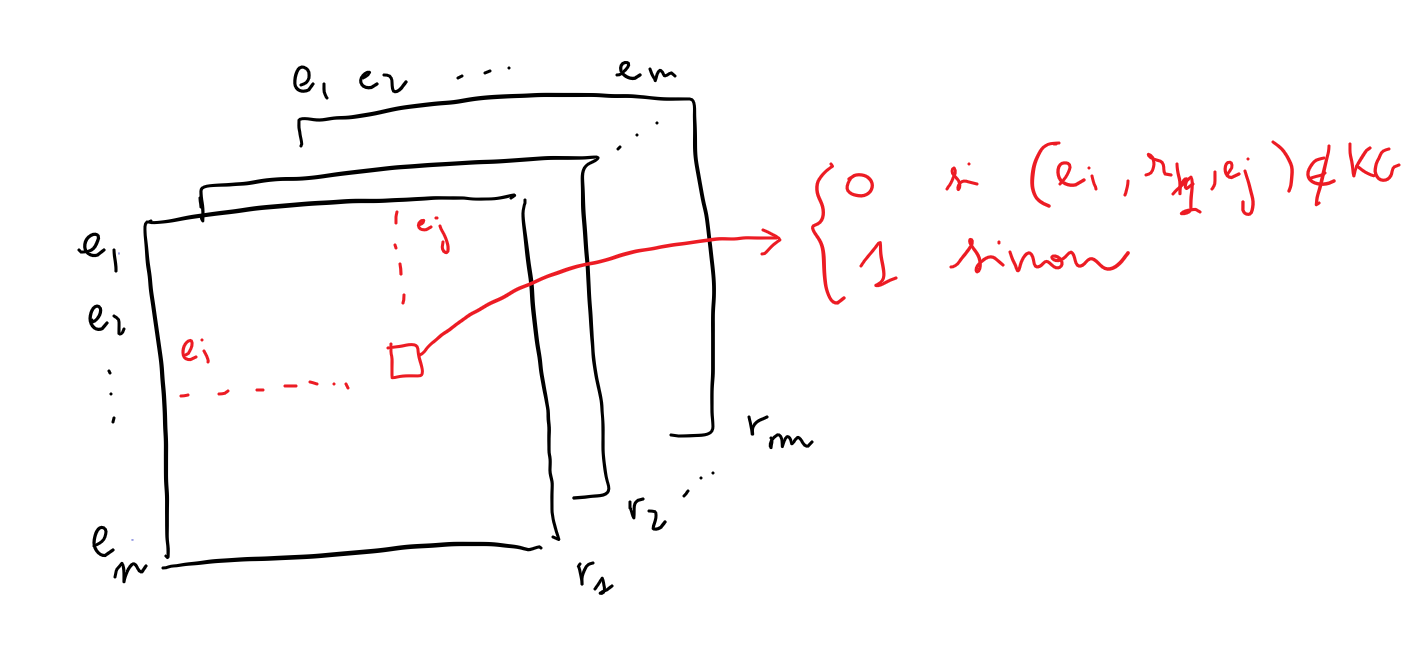
\includegraphics[width=\textwidth]{img/tenseur_adjacence.png}
    \begin{tikzpicture}[
  box/.style={draw=gray, thick, align=center},
  arrow/.style={->, shorten >=3pt, gray!80},
  node/.style={draw=gray, fill=gray!20},
  hnode/.style={draw=accent1, fill=accent1!20},
  snode/.style={draw=accent1, fill=accent1!20, very thick},
  point/.style={circle, draw=gray!80, fill=gray!30, node distance=1cm and 0.5cm, inner sep=0, minimum height=0.25cm},
  spoint/.style={circle, draw=gray!80, fill=gray!30, node distance=1cm and 0.3cm, inner sep=0, minimum height=0.25cm},
  pointA/.style={fill=accent1, draw=accent1},
  pointB/.style={fill=accent2, draw=accent2},
]

\def\l{4}
\def\delta{0.2}
\def\sep{0.1}
\draw[fill=white, draw=black] (0+5*\delta, \l+5*\delta) rectangle (\l+5*\delta, 0+5*\delta);
\draw[fill=white, thick, draw=accent1] (0+3*\delta, \l+3*\delta) rectangle (\l+3*\delta, 0+3*\delta);

\draw[fill=white, draw=black] (0+\delta, \l+\delta) rectangle (\l+\delta, 0+\delta);
\draw[fill=white, draw=black] (0, \l) rectangle (\l, 0);

\draw[draw=accent1, dashed] (0+3*\delta, \l+3*\delta) rectangle (\l+3*\delta, 0+3*\delta);



\node[anchor=north west] at (\l+\sep, -\sep) {$r_1$};
\node[anchor=north west, rotate=45] at (\l+\sep+\delta, 0.5*\delta - \sep) {$\scriptstyle \hdots$};
\node[anchor=north west, rotate=45] at (\l+\sep+3.5*\delta, 3*\delta - \sep) {$\scriptstyle \hdots$};
\node[anchor=north west, text=accent1] at (\l+3*\delta+\sep, 3*\delta-\sep) {$r_k$};
\node[anchor=north west] at (\l+5*\delta+\sep, 5*\delta) {$r_m$};

\node[anchor=east] at (-\sep, \l) {$e_1$};
\node[anchor=east] at (-\sep, \l-6*\sep) {$e_2$};
\node[anchor=east] at (-1.5*\sep, 0.5*\l) {$\vdots$};
\node[anchor=east] at (-\sep, 0) {$e_n$};


\node[anchor=south] at (0+5*\delta, \l+5*\delta+\sep) {$e_1$};
\node[anchor=south] at (0+5*\delta+6*\sep, \l+5*\delta+\sep) {$e_2$};
\node[anchor=south] at (0+5*\delta+0.5*\l, \l+5*\delta+\sep) {$\hdots$};
\node[anchor=south] at (\l+5*\delta, \l+5*\delta+\sep) {$e_n$};

\node[draw=accent1, label={[accent1]15:$\mathcal{T}_{ijk}$}] (ijk) at (0.4*\l, 0.7*\l) {};
\draw[dotted, red] (3*\delta, 0.7*\l) to node[near start, below] {$i$} (ijk);
\draw[dotted, red] (0.4*\l, \l+3*\delta) to node[left, anchor=east] {$j$} (ijk);

\node (eq) at (1.4*\l, 0.9*\l) {};
\draw[->, red] (ijk.315) to[bend right] (eq);

\matrix[matrix of math nodes,left delimiter=\lbrace, right=0.1cm of eq] (mat)
{
0 \textrm{ si } (e_i, r_k, e_j) \notin \mathcal{KG} \\
1 \textrm{ sinon} \\
};

% \node[above left=0.01 of ijk] (r1) {};
% \node[below right=0.01 of ijk] (r2) {};
% \draw[red, dashed] (r1) rectangle (r2);


\end{tikzpicture}
    \caption[Représentation de graphe sous forme de tenseur d'adjacence]{Représentation d'un graphe de connaissance $\KG$ sous forme de tenseur d'adjacence $\cal{T}$.}
    \label{fig:kge-algebric-overview}
\end{figure}

Pour une relation $r \in \Rel$, on note $\bf{X}^{(r)}$ la matrice d'adjacence associée à cette relation : $\bf{X}^{(r)}$ est une matrice booléenne carrée, de dimension $n$ et dont la coordonnée $(i, j)$ contient $1$ si le triplet $(e_i, r, e_j)$ est valide, et $0$ sinon. On peut donc voir $\cal{T}$ comme une collection des matrices $\bf{X}^{(r)}$ : $\cal{T} = [\bf{X}^{(r_1)}, \bf{X}^{(r_2)}, \ldots, \bf{X}^{(r_m)}]$, comme l'illustre la figure  \ref{fig:kge-algebric-overview}. Notons ici que le cas où $\cal{T}_{i, j, k} = 0$ ne signifie pas que le triplet $(e_i, r_k, e_j)$ est invalide : dans l'hypothèse du monde ouvert, un triplet absent du graphe peut être soit invalide, soit inconnu.

Les modèles algébriques présentés dans cette section approximent les matrices $\bf{X}^{(r)}$ par des matrices de rang faible, et extraient de ces approximations des représentations en faible dimension des entités et des relations du graphe. Ils peuvent être rapprochés de techniques de réduction de la dimension comme l'analyse sémantique latente (ou LSA, pour \textit{Latent Semantic Analysis} (ref)), fréquente en traitement des langues naturelles.

Dans toute la suite, $d \in \mathbb{N}$ désigne la dimension des plongements. On choisit généralement $d$ entre 50 et 500.

\subsubsection{RESCAL}

Le modèle RESCAL \cite{rescal} s'appuie sur une factorisation approximative de $\bf{X}^{(r)}$, de rang $d$, qui s'écrit comme suit  :
\begin{equation}
    \bf{X}^{(r)} \approx \bf{E} \cdot \bf{W}_r \cdot \bf{E}^\top
    \label{eq:kge-rescal-factorization}
\end{equation}

Où $\bf{E} \in \R^{n \times d}$ contient la représentation vectorielles des entités, et $\bf{W}_r \in \R^{d \times d}$ modélise l'interaction entre les composants du sujet et de l'objet pour la relation $r$.

Notons $\bf{E} = (\bf{e}_1, \bf{e}_2, \ldots, \bf{e}_n)^\top$ : $\bf{e}_i$ désigne la $i$-ème ligne de $\bf{E}$ et constitue la représentation vectorielle en $d$ dimension de l'entité $e_i$, soit le plongement vectoriel recherché. L'équation \ref{eq:kge-rescal-factorization} présente deux caractéristiques importantes : d'une part, la représentation des entités ne dépend pas de la relation $r$; d'autre part, les entités sont représentées de la même manière selon qu'elles soient sujet ou objet dans la relation. On peut résumer RESCAL avec les deux caractéristiques suivantes :
\begin{itemize}
    \item les entités sont représentés par un vecteur de dimension $d$, qui est le même pour chaque relation et quelle que soit la position de l'entité dans le triplet. 
    \item une relation consiste en une interaction entre les représentations vectorielles de son sujet et de son objet. Cette interaction se traduit mathématiquement par une matrice carrée, a priori non symétrique. La matrice étant asymétrique, le rôle des deux entités impliquées (sujet ou objet) est pris en compte.
\end{itemize}

Ce dernier point est visible lorqu'on ré-écrit l'équation \ref{eq:kge-rescal-factorization} pour un triplet $(e_i, r_k, e_j)$ donné. Notons d'abord $\hat{\bf{X}}^{(r)}$ l'approximation de rang $d$ de $\bf{X}^{(r)}$ :
\begin{equation*}
    \hat{\bf{X}}^{(r)} = \bf{E} \cdot \bf{W}_r \cdot \bf{E}^\top
\end{equation*}
Et $\hat{\cal{T}} = [\hat{\bf{X}}^{(r_1)}, \hat{\bf{X}}^{(r_2)}, \ldots, \hat{\bf{X}}^{(r_m)}]$ l'approximation de rang $d$ du tenseur d'adjacence complet. On peut alors approximer la validité d'un triplet $(e_i, r_k, e_j)$ par :
\begin{equation}
    \hat{\cal{T}}_{i, j, k} = \bf{e}_i^\top \cdot \bf{W}_{r_k} \cdot \bf{e}_j
\end{equation}

Cette équation est fondamentale, puisqu'elle permet d'estimer la validité d'un triplet à partir de ses plongements. On la ré-écrit sous forme plus générique, en interprétant la quantité $\hat{\cal{T}}_{i, j, k}$ comme le \textit{score} associé au triplet $(e_i, r_k, e_j)$ : 
\begin{equation}
    s(h, r, t) = \mathbf{h}^\top \cdot \bf{W}_r \cdot \bf{t}
    \label{eq:rescal}
\end{equation}

Le but est donc d'obtenir des plongements tels que le score $s$ d'un triplet valide soit élevé, et le score d'un triplet invalide soit faible. Pour les obtenir, on définit un programme d'optimisation non-linéaire : les paramètres à entraîner sont les plongements des entités $\bf{E}$ et les $m$ matrices de relation $\bf{R} = \{ \bf{W}_r \}_{r \in \Rel}$. On note $\Theta = (\bf{E}, \bf{R})$ ces paramètres. La fonction de perte mesure l'écart entre le tenseur d'adjacence initial et son approximation de rang $d$, avec un terme de régularisation $g$ supplémentaire :
\begin{equation}
    J(\Theta) = \frac{1}{2} \sum_{r \in \Rel} \left\| \bf{X}^{(r)} - \hat{\bf{X}}^{(r)} \right\|_F^2 + g(\Theta)
    \label{eq:kge-rescal-loss-function}
\end{equation}

On rappelle que $\| \cdot \|_F$ désigne la norme de Frobenius, une norme matricielle définie par $\| \bf{M} \|_F = \sqrt{\sum_{i, j} |M_{i, j}|^2}$. Le terme $g$ est caractérisé par un paramètre $\lambda$ qui indique l'intensité de la régularisation, et défini par :
\begin{equation}
    g(\Theta) = \frac{1}{2} \lambda \left( \| \bf{E} \|_F^2 + \sum_{r \in \Rel} \| \bf{W}_r \|_F^2 \right)
\end{equation}


Pour harmoniser les notations avec les autres modèles de plongement, on peut réécrire la perte $J(\Theta)$ à l'aide de la fonction de score $s$ et de 
%. Pour cela, reprenons 
l'ensemble d'entraînement $\Delta$ défini dans la section \ref{subsec:kge-data} : % constitué de paires $(h, r, t), y$ où $(h, r, t)$ est un triplet et $y$ son label : 0 si le triplet est invalide, 1 sinon. On a alors :
\begin{equation}
    J(\Theta) = \frac{1}{2} \sum_{(h, r, t), y \in \Delta} \left(y - s(h, r, t) \right)^2
    + g(\Theta)
\end{equation}

La perte est donc égale aux carrés de la distance entre le score d'un triplet et son label, plus un terme de régularisation. Muni de cette fonction de perte, l'entraînement des plongements se fait en initialisant aléatoirement les paramètres, puis par descente de gradient sur $J$ jusqu'à atteindre un nombre maximal d'itérations, ou jusqu'à remplir un critère de convergence. Les auteurs \cite{rescal} proposent le critère de convergence suivant :
\begin{equation}
    \frac{\displaystyle \frac{1}{2} \sum_{r \in \Rel} \left\| \bf{X}^{(r)} - \hat{\bf{X}}^{(r)} \right\|_F^2}{\| \cal{T} \|_F^2} < \epsilon
\end{equation}
Dans l'article original, on prend $\epsilon = 10^{-5}$.


Examinons maintenant quelques propriétés du modèle RESCAL. Notons $w_{i, j}$ la coordonnée $i,j$ de $\bf{W}_r$ et $u_i$ la $i$-ème coordonnée d'un vecteur $\bf{u}$, on peut réécrire l'équation~\ref{eq:rescal} sous la forme~:
\begin{equation}
    s(h, r, t) = \sum_{i, j = 1}^{d} h_i \cdot t_j \cdot w_{i, j}
\end{equation}

Ainsi, toutes les combinaisons $h_i t_j$ de $\mathbf{h}$ et de $\mathbf{t}$ apparaissent dans la fonction de score, avec un coefficient $w_{i, j}$. En ce sens, RESCAL propose une expressivité maximale et permet de modéliser une large palette de relations. Par exemple, si $\mathbf{W_r}$ est symétrique (c'est-à-dire, $\mathbf{W}_r = \mathbf{W}_r^\top$), on a $w_{i,j} = w_{j, i}$ pour tous $i, j = 1, \ldots, d$, et donc :

\begin{equation}
    s(h, r, t) = \sum_{i, j = 1}^{d} \mathbf{h_i \cdot t_j} \cdot d_{i, j}
    =  \sum_{i, j = 1}^{d} \mathbf{h_j \cdot t_i} \cdot w_{j, i}
    =  \sum_{i, j = 1}^{d} \mathbf{h_j \cdot t_i} \cdot w_{i, j}
    = s(t, r, h)
\end{equation}

Une matrice symétrique induit donc une fonction de score symétrique elle aussi; cela permet de modéliser des relations symétriques. Inversement, si $\mathbf{W_r}$ est antisymétrique (c'est-à-dire, $\mathbf{W}_r = -\mathbf{W}_r^\top$), on aura une fonction de score antisymétrique, ce qui permet de modéliser une relation antisymétrique.

Cette expressivité se paie toutefois par un nombre élevé de paramètres ($d^2$ par relation) : cela demande plus de mémoire que les modèles décrits dans les sections suivantes, et surtout cela complique l'entraînement du modèle, en compliquant la régularisation et favorisant le sur-apprentissage (ref). Pour ces raisons, on n'utilise pas RESCAL dans ce travail, mais deux modèles apparentés : DistMult et ComplEx, présentés dans les deux sections suivantes.

\subsubsection{DistMult}

DistMult \cite{distmult}, bien qu'il ne soit pas présenté comme tel par ses auteurs, peut être vu comme une simplification de RESCAL pour le rendre plus facile à entraîner et moins sujet au sur-apprentissage. Pour cela, on conserve comme fonction de score un produit trilinéaire entre les plongements des éléments du triplets  (équation~\ref{eq:rescal}), mais on impose que la matrice $\mathbf{W_r}$ soit diagonale – soit $d$ paramètres par relation au lieu de $d^2$. Cela revient à représenter une relation $r$ par un vecteur $\mathbf{r}$ de dimension $d$, et à poser $\mathbf{W_r = I_{d\times d} \cdot r}$. La fonction de score s'écrit donc :
\begin{equation}
    \label{eq:distmult}
    s(h, r, t) = \mathbf{h^\top \cdot I_{d\times d}r \cdot t}
\end{equation}

Ce qui se réécrit sous forme non-matricielle :
\begin{equation}
    s(h, r, t) = \sum_{i=1}^{d} h_i r_i t_i
    \label{eq:kge-distmult-scorenv}
\end{equation}

Ainsi, la fonction de score peut être vue comme un produit scalaire à trois vecteurs. Comparé à RESCAL, l'expressivité est très réduite : seule les combinaisons de la forme $\mathbf{h_i t_i}$ sont utilisées pour le calcul du score. De plus, $s$ est toujours symétrique, donc le sujet et l'objet d'un triplet ne sont pas différenciés.

% L'équation \ref{eq:kge-distmult-scorenv} permet d'interpréter la fonction de score de DistMult comme une mesure de similarité entre le sujet $h$ et l'objet $t$, pondérée en fonction de la relation $r$ considérée. En effet, le terme $\bf{h^\top \cdot t}$ s'interprète comme une similarité cosinus sans normalisation, et chaque coefficient $r_i$ indique le poids à accorder à chaque dimension.


L'entraînement de DistMult se fait avec une fonction de perte spécifique, la perte par marge maximale, qui s'écrit comme suit :
\begin{equation}
    J(\Theta) = \sum_{(h, r, t) \in \Delta_+} \sum_{(h', r', t') \in \Delta_-} \lfloor \gamma + s(h', r', t') - s(h, r, t) \rfloor_+
    \label{eq:kge-distmult-maxmarginloss}
\end{equation}
Pour rappel, $\lfloor \cdot \rfloor_+$ désigne la partie positive, c'est-à-dire que $\lfloor x \rfloor_+$ vaut $x$ si $x > 0$, et vaut zéro sinon. Pour interpréter cette perte, considérons un triplet valide $u \in \Delta_+$ et un triplet invalide $u' \in \Delta_-$. L'objectif d'un modèle est de maximiser le score de $u$ et de minimiser celui de $u'$. Si on pose $\Delta s = s(u) - s(u')$ (c'est l'écart entre le score de $u$ et celui de $u'$), cet objectif revient alors à maximiser $\Delta s$. Le terme de la somme dans l'équation \ref{eq:kge-distmult-maxmarginloss} s'écrit :
\begin{equation}
    j(u, u') = \lfloor \gamma - \Delta s \rfloor_+
\end{equation}
Ainsi, la perte associée à $u$ et $u'$ est nulle si $\Delta s \geq \gamma$, et vaut $\gamma - \Delta s$ sinon. L'objectif du modèle est donc de séparer les scores des triplets valides des scores des triplets invalides, et ce d'une marge au moins égale à $\gamma$. Ce choix de fonction de score est cohérent avec l'usage premier d'un modèle de plongement, qui est de prédire la validité d'un triplet inconnu : pour cet usage, l'enjeu est précisément de pouvoir distinguer les scores des triplest valides de ceux des triplets invalides.

\subsubsection{ComplEx}
\label{subsec:complex}

ComplEx (ref) est une extension de DistMult dans l'espace complexe. Comme RESCAL, il s'appuie sur une décomposition de la matrice d'adjacence $\bf{X}^{(r)}$ associée à la relation $r$ pour en réduire la dimension.

Pour motiver la conception de ComplEx, les auteurs s'interrogent sur les fondements mathématiques de la factorisation de $\bf{X}^{(r)}$. Avant réduction de la dimension, la décomposition qui sert de base à DistMult peut s'écrire :
\begin{equation}
    \bf{X}^{(r)} = \bf{E} \cdot \bf{W}_r \cdot \bf{E}^\top
    \label{eq:kge-complex-spectral}
\end{equation}
Avec $\bf{E} \in \R^{n \times n}$ et $\bf{W}_r \in \R^{n \times n}$ une matrice diagonale : il s'agit de la diagonalisation d'une matrice réelle symétrique sur une base orthonormée. Toutefois, cette décomposition n'existe que dans le cas particulier où $\bf{X}^{(r)}$ est symétrique : en effet, les valeurs propres d'une matrice réelle symétrique sont réelles, et leurs sous-espaces propres sont orthogonaux, donc le théorème spectral s'applique.

En revanche, la décomposition précédente n'est pas possible dans le cas général où $\bf{X}^{(r)}$ n'est pas symétrique. Dès qu'une relation $r$ n'est pas symétrique, RESCAL effectue donc deux approximations successives : d'abord par la décomposition \ref{eq:kge-complex-spectral}, et ensuite par la réduction de dimension (c'est-à-dire, lorsqu'on ne garde que les $d$ premières composantes de $\bf{E}$ et $\bf{W}_r$). Pour éliminer la première approximation, on pourrait utiliser la décomposition en valeur singulière (SVD, pour \textit{Singular Value Decomposition}), qui s'écrit :
\begin{equation}
    \bf{X}^{(r)} = \bf{U} \cdot \bf{W}_r \cdot \bf{V}^\top
\end{equation}
Avec $\bf{U}, \bf{V} \in \R^{n \times n}$. Dans ce cas, on a $\bf{U \neq V}$ en général, on perd donc une propriété essentielle de la décomposition précédente : une entité possède une représentation unique qu'elle soit sujet ou objet dans la relation. 

ComplEx vise à concilier ces deux exigences : obtenir une représentation unique des entités, indépendante de leur rôle dans le triplet – comme dans la décomposition en valeurs propres des matrices symétriques; et pouvoir représenter des matrices non-symétriques, comme dans la décomposition en valeurs singulières. Pour cela, le modèle utilise la diagonalisation sur une base de vecteurs propres, comme l'équation \ref{eq:kge-complex-spectral}, dans le cas général où $\bf{X}^{(r)}$ n'est pas symétrique : dans ce cas, $\bf{E}$ et $\bf{W}_r$ ne sont plus nécessairement réelles, et la décomposition s'écrit :
\begin{equation}
    \bf{X}_r = \bf{E} \cdot \bf{W}_r \cdot \compconj{\bf{E}}^\top
    \label{eq:kge-complex-main}
\end{equation}
Avec $\bf{E} \in \mathbb{C}^{n \times n}$ désormais complexe, et $\bf{W}_r \in \mathbb{C}^{n \times n}$ une matrice diagonale complexe qui contient les valeurs propres de $\bf{X}^{(r)}$, classées dans l'ordre décroissant de leurs modules. En gardant alors les $d \times d$ premières coordonnées de $\bf{W}_r$ pour former les matrices $\bf{W}_r^{(d)} \in \mathbb{C}^{d \times d}$ et $\bf{E}^{(d)} \in \mathbb{C}^{n \times d}$, on obtient une approximation de $\bf{X}_r$ de dimension $d$ :
\begin{equation}
    \bf{X}_r \approx \bf{E}^{(d)} \cdot \bf{W}_r^{(d)} \cdot \compconj{ \bf{E}^{(d)}}^\top
\end{equation}

La matrice $\bf{X}^{(r)}$ devant être réelle, son approximation en basse dimension est projetée dans $\R$ en ne considérant que la partie réelle de $\bf{E}^{(d)} \cdot \bf{W}_r^{(d)} \cdot \compconj{ \bf{E}^{(d)}}^\top$. Autrement dit, la fonction de score de ComplEx peut s'écrire :
\begin{equation}
    \eta(h, r, t) = \Re(\bf{h^\top \cdot W}_r \cdot \compconj{\bf{t}})
\end{equation}
Avec $\bf{h, t} \in \mathbb{C}^d$ des vecteurs complexes, et $\bf{W}_r$ une matrice complexe diagonale de dimension $d \times d$. Si on note $\eta$ ce score et non $s$, c'est parce que ComplEx fait un choix de modélisation légèrement différent des modèles précédents. En effet, plutôt que de prédire directement des valeurs entre 0 et 1, on autorise les coefficients de $\Re(\bf{h^\top \cdot W}_r \cdot \compconj{\bf{t}})$ à prendre n'importe quelle valeur dans $] -\infty, +\infty [$, et on ramène ensuite le score dans $[0, 1]$ à l'aide de la fonction logistique : $\sigma : z \mapsto (1 + e^{-z})^{-1}$, soit une fonction de score finalement égale à $s = \sigma \circ \eta$:
\begin{equation}
    s(h, r, t) = \sigma \left( \Re(\bf{h^\top \cdot W}_r \cdot \compconj{\bf{t}}) \right)
\end{equation}

Un avantage théorique de la fonction de score de ComplEx par rapport aux précédentes est qu'elle est capable d'être symétrique, antisymétrique ou ni l'un ni l'autre, selon la position de $\bf{W}_r$ dans l'espace complexe. Considérons d'abord le cas où $\bf{W}_r$ est réelle ($\bf{W}_r \in \R^{d \times d}$). On a :
\begin{align}
    \eta(h, r, t) &= \Re(\bf{h^\top \cdot W}_r \cdot \compconj{\bf{t}}) \\
    &= \Re\left((\compconj{\bf{h^\top \cdot W}_r \cdot \compconj{\bf{t}}})^\top\right) \label{eq:complex-symmetric-1} \\
    &= \Re\left( \compconj{\compconj{\bf{t}}^\top \cdot \compconj{\bf{W}_r}^\top \cdot 
    \compconj{\bf{h^\top}}^\top}\right) \label{eq:complex-symmetric-2} \\
    &= \Re\left(\bf{t}^\top \cdot \bf{W}_r \cdot \compconj{\bf{h}}\right) \label{eq:complex-symmetric-3} \\
    &= \eta(t, r, h)
\end{align}
\ref{eq:complex-symmetric-1} est vraie car la partie réelle est invariante par conjugaison, et \ref{eq:complex-symmetric-3} parce que $\bf{W}_r$ est réelle et symétrique. On ramène alors le score dans l'intervalle $[0, 1]$, et on obtient :
\begin{equation}
    s(h, r, t) = s(t, r, h)
\end{equation}
Ainsi, $s$ attribue le même score à un triplet et à son symétrique lorsque le plongement de la relation associée est réel, on peut donc modéliser plus fidèlement une relation symétrique. 
Si un triplet $(h, r, t)$ est valide et présent à l'entraînement, le modèle sera entraîné pour maximiser $s(h, r, t)$; or, sous réserve que $\bf{W}_r$ soit réelle, on aura $s(t, r, h) = s(h, r, t)$ et donc on aura bien l'équivalence : $(h, r, t) \text{ est valide} \iff (t, r, h) \text{ est valide}$.

Inversement, si $\bf{W}_r$ est imaginaire pure, c'est-à-dire $\bf{W}_r \in i\R$, on aura $\compconj{\bf{W}_r} = - \bf{W}_r$; en injectant ce résultat dans l'équation \ref{eq:complex-symmetric-2}, on aura :
\begin{equation}
    \eta(h, r, t) = - \eta(t, r, h)
\end{equation}
Ce qui, une fois ramené dans $[0, 1]$, donne :
\begin{equation}
    s(h, r, t) = 1 - s(t, r, h)
\end{equation}
Donc un plongement imaginaire pur modélisera des relations antisymétriques, puisqu'un score proche de 1 pour le triplet $(h, r, t)$ impliquera nécessairement un score proche de 0 pour le symétrique $(t, r, h)$. 

Enfin, dans le cas général où $\bf{W}_r$ n'est ni réelle, ni imaginaire pure, la relation $r$ modélisée ne sera ni symétrique, ni antisymétrique.  Évidemment, il s'agit là de propriétés \textit{théoriques} du modèle : en particulier, ces propriétés ne sont utiles qu'à la condition que le modèle soit capable de faire converger les plongements des relations symétriques vers l'espace réel, et les plongements des relations antisymétriques vers l'espace des imaginaires purs. 
%
Notons toutefois que la fonction de score est continue en $\bf{W}_r$ : même si les conditions de symétrie ($\bf{W}_r \in \R^{d \times d}$) ou d'antisymétrie ($\bf{W}_r \in i\R^{d \times d}$) ne sont pas exactement respectées, la fonction de score peut s'approcher des propriétés de symétrie ($\eta(h, r, t) \approx \eta(t, r, h)$) ou d'antisymétrie ($\eta(h, r, t) \approx - \eta(t, r, h)$).%, ce qui facilite l plus $\bf{W}_r$ n'est pas exactement imainaire pure mais s'en rapproche, la fonction de score se rapprochera également

% Toutefois, cela indique une expressivité \textit{a priori}, que n'ont ni TransE, ni DistMult. En effet, pour TransE, une relation symétrique devrait vérifier $\bf{h + r - t} \approx 0$ et $\bf{t + r - h} \approx 0$, pour tous les plongements $\bf{h, t}$; en injectant la seconde équation dans la première, on obtient $\bf{h + r + r} \approx h, \forall \bf{h}$, soit $\bf{r \approx -r}$ et donc $\bf{r} \approx 0$. Ainsi,  une relation modélisée par TransE n'est pas symétrique, sauf dans le cas particulier où $\bf{r}$ est nul. Dans le cas de DistMult, toutes les relations sont symétriques.


\subsection{Modèles translationnels : TransE et ses variantes}
\label{subsec:kge-models-transx}

On introduit ici une seconde approche, davantage géométrique, que l'on présente à travers l'exemple des modèles translationnels. Un modèle géométrique abandonne la référence au graphe vu comme un tenseur d'adjacence. Il est caractérisé par deux éléments : d'une part, des plongements vectoriels $\bf{E} = \{ \bf{e} \}_{e \in \Ent} \subset \R^d$ représentant les entités; d'autre part, une famille d'opérateurs géométriques $\{ F_r \}_{r \in \Rel}$ qui combinent les plongements de deux entités. % en fonction d'une relation. 
En appliquant l'opérateur $F_r$ aux plongements $\bf{h}$ et $\bf{t}$, on obtient un nombre réel positif appelé l'\textit{énergie} du triplet $(h, r, t)$ et noté $E(h, r, t)$. L'objectif d'un modèle de plongement géométrique est de minimiser l'énergie des triplets valides, et de maximiser celle des triplets invalides.

Dans cette section, on examine une unique famille de modèles géométriques, les modèles translationnels. L'opérateur $F_r$ d'un modèle translationnel est précisément la translation du sujet d'un triplet vers l'objet du triplet, la translation étant paramétrée par la relation considérée. Le premier de ces modèles a été TransE \cite{bordes2013translating}; il a inspiré un grand nombre de variantes dont on présente deux exemples : TransH \cite{transh} et TransD \cite{transd}.

\subsubsection{TransE \cite{bordes2013translating}}

L'idée fondamentale de TransE est de représenter une relation entre deux entités comme une translation entre leurs plongements. Une translation dans $\R^d$ est une opération linéaire qui consiste intuitivement à «déplacer» un point vers un autre. La distance et le sens de ce déplacement sont caractérisées par un vecteur $\bf{u} \in \R^d$; pour un tel vecteur $\bf{u}$, la translation associée s'écrit:
\begin{equation}
    T_\bf{u} : \bf{x} \mapsto \bf{u + x}
\end{equation}

Dans TransE, chaque relation est associée à un vecteur $\bf{r}$ à $d$ dimensions, et donc à une translation $T_r$. Un triplet $(h, r, t)$ est valide si le translaté du plongement de $h$ par $T_r$ est proche ou égal au plongement de $t$ :
\begin{equation}
    (h, r, t) \text{ est valide } \iff T_r(\bf{h}) \approx \bf{t} 
\end{equation}

Les auteurs défendent l'idée que les relations hiérarchiques sont le type de relation fondamentale d'un graphe de connaissance, et que la translation est une approximation naturelle pour modéliser une hiérarchie. % Ainsi, la représentation naturelle d'un arbre en dimension 2 
De plus, ils remarquent que les plongements lexicaux Word2Vec \cite{mikolov2013distributed} traduisent naturellement certaines relations \textit{one-to-one} comme des translations. Dans l'article original de Word2Vec \cite{mikolov2013distributed}, les auteurs remarquent la fameuse propriété de leur modèle :
\begin{equation}
    \texttt{vec(Berlin) - vec(Germany)} \approx 
    \texttt{vec(Paris) - vec(France)}
\end{equation}
Ce qui revient à dire que la relation «être capital de» se traduit géométriquement par une translation entre le sujet et l'objet. Dans le cas de Word2Vec, il s'agit d'une propriété émergente du modèle, qui n'étais pas attendue par ses auteurs; pour TransE, on impose au contraire cette propriété comme point de départ de la modélisation.

\begin{figure}
    \centering
    \begin{tikzpicture}
[   cnode/.style={draw=gray!40,fill=gray!20,text width=1mm, scale=0.3, circle},
    rnode/.style={draw=black,fill=#1,minimum width=6mm, minimum height=5mm, rectangle},
    rline/.style={red,thick, ->}
]
    
    \def\rx{5};
    \def\ry{2};
    
    \def\ox{0.5*\rx};
    \def\oy{0.5*\ry};
    \node (origin) at (\ox, \oy) {};
    \node (x) at (\ox + 1 * \rx, \oy) {};
    \node (y) at (\ox - 0.25*\rx, \oy-1.3*\ry) {};
    \node (z) at (\ox, \oy+2) {};
    
    \draw[gray!70, ->] (origin.center) -- (x);
    \draw[gray!70, ->] (origin.center) -- (y);
    \draw[gray!70, ->] (origin.center) -- (z);
    
    \node[cnode, label={100:\texttt{China}}] (a1) at (-0.5, 0.1) {};
    \node[cnode, label={270:\texttt{United\_States}}] (a2) at (1, -0.3)   {};
    \node[cnode, label={270:\texttt{France}}] (a3) at (0.7, 0.4)  {};
    
    \node[cnode, label={\texttt{Beijing}}] (b1) at (-0.5+\rx, 0.1+\ry)  {};
    \node[cnode, label={10:\texttt{Washington,\_D.C.}}] (b2) at (1+\rx, -0.3+\ry) {};
    \node[cnode, label={45:\texttt{Paris}}] (b3) at (0.7+\rx, 0.4+\ry)  {};
    
    \draw[rline] (a1) -- (b1);
    \draw[rline] (a2) -- node[below, sloped]{\texttt{dbo:capital}} (b2);
    \draw[rline] (a3) -- (b3);
    
    % \draw[->,blue,thick] (0,0) -- node[above, sloped]{$\mathbf{h}$} % (1, 1.8);
    % \draw[->,red, thick] (0,0) -- node[above, sloped]{$\mathbf{t}$} % (3, 1.2);
    % \draw[->] (1,1.8) -- node[above, sloped]{$\mathbf{r}$} (2.9, % 1.25);
    
    % \draw[->] (0,0) -- (4,0);
    % \draw[->] (0,0) -- (-0.5, -0.75);
    % \draw[->] (0,0) -- (0,2);
    
    % \node at (2, -1.5) {$(h, r, t) \in \mathcal{KG} \iff \mathbf{h} + \mathbf{r} \approx \mathbf{t} $}
\end{tikzpicture}
    \caption[Principe du modèle TransE]{Modèle de plongement TransE. La relation \texttt{dbo:capital} est représentée par une translation, en rouge, qui relie les plongements des sujets aux plongement des objets.}
    \label{fig:transe-intuition}
\end{figure}

Mathématiquement, la relation $T_r(\bf{h}) \approx \bf{t}$ est quantifiée en mesurant la distance euclidienne entre le translaté $T_r(\bf{h})$ et l'objet $\bf{t}$, ce qui définit l'énergie associée au triplet :
\begin{equation}
    E_\Theta(h, r, t) =  d_\text{euc}(T_r(\bf{h}), \bf{t})
    \label{eq:transe-mainvar}
\end{equation}
Ce qui est plus généralement écrit :
\begin{equation}
    E_\Theta(h, r, t) = \| \mathbf{h + r - t} \|_2
    \label{eq:transe-main}
\end{equation}

Le nombre de paramètres est donc $d \times (n + m)$, linéaire en le nombre d'éléments du graphe. 

La force de TransE réside dans sa simplicité théorique et son faible nombre de paramètres. Toutefois, cette simplicité se paye par une faible expressivité, qui limite sa capacité à modéliser des relations autres que \textit{one-to-one} :
\begin{itemize}
    \item relation \textit{many-to-one} : si plusieurs entités $h_1, h_2, \ldots, h_k$ sont reliées à une même entité $t$ par une relation $r$, alors les translatés $\mathbf{h_i + r}$ doivent tous être égaux, donc $\mathbf{h_1  = h_2 = \ldots = h_k}$;
    \item relation \textit{one-to-many} : comme au-dessus, si $h$ est lié par $r$ à plusieurs entités $t_1, \ldots, t_k$, alors nécessairement $\mathbf{t_1 = t_2 = \ldots = t_k}$;
    \item relations symétriques : si $r$ est symétrique, c'est-à-dire $h  \overset{r} \rightarrow t \implies t   \overset{r} \rightarrow h$, alors la translation de la translation par $r$ doit donner l'élément de départ, donc $\mathbf{r} = 0$
\end{itemize}

\begin{figure}[h]
    \centering
    \begin{tikzpicture}
        [
            neuron/.style={draw=black!40, fill=black!20, circle, scale=0.5},
            rel/.style={draw=black}
        ]
    \def\ox{0.5}
    \def\oy{0.5}
	\node [neuron, label={180:$h_1$}] (0) at (0*\ox, 3*\oy) {};
	\node [neuron, label={180:$h_2$}] (1) at (0*\ox, 2*\oy) {};
	\node at (0*\ox, 1.2*\oy) {$\vdots$};
	\node [neuron, label={180:$h_m$}] (3) at (0*\ox, 0*\oy) {};
	\node [neuron, label={0:$t$}] (4) at (2*\ox, 1.5*\oy) {};
	\node [neuron, label={180:$h$}] (10) at (0*\ox, -2.5*\oy) {};
	\node [neuron, label={0:$t_1$}] (5) at (2*\ox, -1*\oy) {};
	\node [neuron, label={0:$t_2$}] (6) at (2*\ox, -2*\oy) {};
	\node at (2*\ox, -2.8*\oy) {$\vdots$};
	\node [neuron, label={0:$t_m$}] (7) at (2*\ox, -4*\oy) {};
	\node [neuron, label={180:$e$}] (8) at (0*\ox, -6*\oy) {};
	\node [neuron, label={0:$e'$}] (9) at (2*\ox, -6*\oy) {};
	\node [label={180:{\textit{many-to-one}}}] (11) at (-2*\ox, 1.5*\oy) {};
	\node [label={180:{\textit{one-to-many}}}] (12) at (-2*\ox, -2.5*\oy) {};
	\node [label={180:{symétrique}}] (13) at (-2*\ox, -6*\oy) {};
	\node[label={0:$\implies \mathbf{h_1} = \mathbf{h_2} = \ldots = \mathbf{h_m}$}] (14) at  (4*\ox, 1.5*\oy) {};
	\node[label={0:$\implies \mathbf{t_1} = \mathbf{t_2} = \ldots = \mathbf{t_m}$}] (15) at  (4*\ox, -2.5*\oy) {};
	\node[label= {0:$\implies \mathbf{r} = \mathbf{0}$}] (16) at  (4*\ox, -6*\oy) {};
		
		\draw [style=rel, ->] (0) to node[above]{$r$} (4);
		\draw [style=rel, ->] (1) to (4);
		\draw [style=rel, ->] (3) to (4);
		\draw [style=rel, bend right, ->] (8) to node[below]{$r$} (9);
		\draw [style=rel, ->] (10) to node[above]{$r$} (5);
		\draw [style=rel, ->] (10) to (6);
		\draw [style=rel, ->] (10) to (7);
		\draw [style=rel, bend left, <-] (8) to (9);
        \end{tikzpicture}
    \caption[Limites du modèle TransE]{Limites du modèle TransE, pour les relations qui ne sont pas \textit{one-to-one}.}
    \label{fig:transe-limitation}
\end{figure}

Pour résoudre ces problèmes, plusieurs modèles basés sur TransE ont été proposés. Leur idée consiste à ajouter une étape préalable à la translation : le plongement d'une entité $e$ est d'abord envoyé dans un nouvel espace, qui dépend de $r$ et éventuellement de $e$, avant d'être translaté dans ce nouvel espace.

Ainsi, on peut définir le cadre général suivant pour décrire un modèle translationnel :
\begin{itemize}
    \item une fonction de transformation $F_{e, r} : \mathbb{R}^d \rightarrow \mathbb{R}^{k}$
    \item une fonction d'énergie $E_\Theta(h, r, t) = \| F_{h, r}(\mathbf{h}) + \mathbf{r} - F_{t, r}(\mathbf{t}) \|_2 $
\end{itemize}

Dans le cas de TransE, la fonction de transformation est la fonction identité :
\begin{equation}
    \forall e, r, F_{e, r} : \bf{u} \mapsto \bf{u}
\end{equation}

On présente maintenant deux modèles basés sur cette idée, le premier utilisant comme fonction de transformation la projection sur un hyperplan, le second une application linéaire qui dépend du triplet considéré.

\FloatBarrier


\subsubsection{TransH \cite{fu2014learning}}

\begin{figure}[hbt]
    \centering
    \begin{tikzpicture}
\def\rep{3};
\def\size{1};
\def\px{-0.5*\size};
\def\py{1.5*\size};
\def\pz{-.5*\size};
\def\hplane{(\px, \py, \pz)};

\def\hsize{2};
\def\vsize{2};
\def\offset{0.5};

\tikzmath{
    \base=2;
    \rx=1*\base;
    \ry=0.5*\base;
    \rz=0.5*\base;
    % h_p
    \hp1=-0.5;
    \hp2=0.5;
    \hp3=-(\hp1*\rx+\hp2*\ry)/\rz;
    \h1=\hp1+\rx;
    \h2=\hp2+\ry;
    \h3=\hp3+\rz;
    % t_p
    \tp1=0.5;
    \tp2=1;
    \tp3=-(\tp1*\rx+\tp2*\ry)/\rz;
    \t1=\tp1+\rx;
    \t2=\tp2+\ry;
    \t3=\tp3+\rz;
    % v
    \v1=-sqrt(((\rx)^2) / ((\rx)^2 + (\rz)^2));
    \v2=0;
    \v3=sqrt(((\rz)^2) / ((\rx)^2 + (\rz)^2));
    % u
    \u1=-\ry / (\rx - (\v1 * \rz) / \v3);
    \u2=1;
    \u3=-\u1*\v1/\v3;
}

\newcommand{\makeplane}{
    % Make axis
    \node (o) at (0, 0, 0) {};
    \node (x) at (\rep, 0, 0) {};
    \node (y) at (0, \rep, 0) {};
    \node (z) at (0, 0, \rep) {};
    
    \draw[axis] (o.center) -- (x);
    \draw[axis] (o.center) -- (y);
    \draw[axis] (o.center) -- (z);
    
    % Make plane
    \filldraw[plane] 
    (\hsize*\v1, \hsize*\v2, \hsize*\v3)
    --  ++(\vsize*\u1, \vsize*\u2, \vsize*\u3)
    -- ++(-2*\hsize*\v1, -2*\hsize*\v2, -2*\hsize*\v3)
    -- ++(-\vsize*\u1, -\vsize*\u2, -\vsize*\u3)
    -- node[below, accent1, sloped, near end] {$H_r$} cycle;
}

\begin{scope}
    % Make axis
    \makeplane
    
    \node[node=accent1, label={[accent1]$\bf{h_\bot}$}] (hp) at (\hp1,\hp2,\hp3) {};
    \node[node=black, label={$\bf{h}$}] (h) at (\h1,\h2,\h3) {};
    \draw[accent1, thick, ->] (h) -- (hp);
    
    \node[node=accent1, label={[accent1]$\bf{t_\bot}$}] (tp) at (\tp1,\tp2,\tp3) {};
    \node[node=black, label={$\bf{t}$}] (t) at (\t1,\t2,\t3) {};
    \draw[accent1, thick, ->] (t) -- (tp);
\end{scope}

\begin{scope}[xshift=7.5cm]
    % Make axis
    \makeplane
    
    \node[node=black, label={$\bf{h_\bot}$}] (hp) at (\hp1,\hp2,\hp3) {};
    % \node[node=gray, label={$h$}] (h) at (\h1,\h2,\h3) {};
    % \draw[gray, thin, ->] (h) -- (hp);
    
    \node[node=black, label={$\bf{t_\bot}$}] (tp) at (\tp1,\tp2,\tp3) {};
    % \node[node=gray, label={$t$}] (t) at (\t1,\t2,\t3) {};
    % \draw[gray, thin, ->] (t) -- (tp);
    
    \node (hr) at (\tp1-\offset*\u1,\tp2-\offset*\u2,\tp3-\offset*\u3) {};
    
    \draw[accent1, thick, ->] (hp) -- node[sloped, below] {$\bf{r}$} (hr.center);
    \draw[thin, accent2, <->] (hr.center) -- node[accent2, near start,right] {$E(h, r, t)$} (tp);
\end{scope}
\end{tikzpicture}
    \caption[Principe général de TransH]{Principe général de TransH : pour calculer le score d'un triplet $(h, r, t)$, on commence par projeter $\bf{h}$ et $\bf{t}$ sur l'hyperplan $H_r$, puis on translate $\bf{h}$. Le score du triplet est égal à la distance entre le translaté de $\bf{h}$ et $\bf{t}$.}
    \label{fig:transh}
\end{figure}

Le premier de ces modèles est TransH, qui associe un hyperplan $H_r$ à chaque relation $r$, et projette les plongements des entités sur cet hyperplan avant de procéder à la translation. 

Un hyperplan $H$ de $\R^d$ est un sous-espace vectoriel de $\R^d$, de dimension $d-1$ : c'est la généralisation en $n$ dimensions d'un plan dans un espace de dimension 3. Un hyperplan $H$ se caractérise par son vecteur normal $\bf{n}$ : un vecteur $\bf{u}$ appartient à $H$ si et seulement s'il est orthogonal à $\bf{n}$. On peut donc associer à tout vecteur non-nul $\bf{n}$ un hyperplan $H_\bf{n}$ :
\begin{equation}
    H_\bf{n} = \{ \bf{x} \in \R^d : \bf{x \cdot n = 0_d} \} \subset \R^d
    \label{eq:kge-transh-hyperplane}
\end{equation}

On note $p_{\bf{n}}$ le projecteur orthogonal associé à un hyperplan $H_{\bf{n}}$, qui s'écrit : %$p_H$ projette les vecteurs de $\R^d$ sur $H_{\bf{n}}$, de sorte à ce que $\bf{x} - p_{\bf{n}}(\bf{x})$ soit orthogonal à $H_{\bf{n}}$. %à $p_H(\bf{x})$
Il s'écrit :
\begin{equation}
    p_{\bf{n}}(\bf{x}) = \bf{x - (n^\top x) \cdot n}
\end{equation}

Dans le cas de TransH, on apprend comme dans TransE des plongements vectoriels de dimension $d$ pour toutes les entités et les relations du graphe, mais on y ajoute un vecteur normal $\bf{w}_r$ pour chaque relation $r$. Ce vecteur normal permet d'associer à chaque relation $r$ un hyperplan $H_r$, selon l'équation \ref{eq:kge-transh-hyperplane}.
%
Pour une relation $r$ donnée, et une entité $e$, on note $\bf{e_\bot} = p_{\bf{w}_r}(\bf{e})$ le projeté orthogonal du plongement de $e$ sur l'hyperplan $H_r$. On impose de surcroît $\bf{r} \in H_r$ pendant l'entraînement.

L'énergie d'un triplet s'écrit alors :
\begin{equation}
    E(h, r, t) = \| \bf{h_\bot + r - t_\bot} \|_2
    \label{eq:kge-transh-main}
\end{equation}
Si l'on remplace les projetés orthogonaux par leurs formules, on retrouve l'équation de TransE avec un terme correcteur $\bf{w}_r^\top \cdot (\bf{h - t}) \cdot \bf{w}_r$:
\begin{equation}
    E(h, r, t) = \left\| \bf{h + r - t} - \left( \bf{w}_r^\top \cdot (\bf{h - t}) \cdot \bf{w}_r \right) \right\|_2
    \label{eq:kge-transh-long}
\end{equation}

\begin{figure}[hbt]
    \centering
    \begin{tikzpicture}
[
scale=0.8,
separation/.style={-, draw=gray!40, dashed},
proja/.style={-, draw=red!20, thin},
projb/.style={-, draw=blue!20}
]

\node  (0) at (0, 0) {};
\node (1) at (0, 2) {};
\node (2) at (2, 3) {};
\node (3) at (4, 4) {};
\node (4) at (3, -1) {};
\node (5) at (3, 1) {};
\node (6) at (7, 3) {};
\node (7) at (7, 1) {};
\node (8) at (4, 2) {};
\node (9) at (4, -2) {};
\node (10) at (7, -3) {};
\node (11) at (3, -5) {};
\node (12) at (0, -4) {};
\node (13) at (-2, 4) {};
\node (14) at (-2, 6) {};
\node (15) at (-6, 2) {};
\node (16) at (-6, 4) {};
%\node (17) at (3, -8) {};
\node (18) at (7, -6) {};
\node (19) at (9, -4.75) {};
\node (20) at (0, -7) {};
\node (21) at (-4, -5) {};
\node (22) at (-8, -2.75) {};
\node (23) at (-8, 6) {};
\node (24) at (-4, 8) {};
\node (25) at (0, 8) {};
\node (26) at (0, 4) {};
\node (27) at (-8, -4) {};
\node (28) at (-9.5, -3.5) {};
\node (29) at (-13, 1) {};
\node (30) at (-8, -4.75) {};
\node (31) at (-7.1, -4.35) {};
\node (32) at (-2, -1) {};
\node (45) at (5, -7) {};
\node (46) at (9, -2.75) {};

\fill [plane-content=accent2] (27.center) -- (23.center) -- (24.center) -- (25.center) -- (26.center) -- (0,0) -- (32.center) -- cycle;
\fill [plane-content=accent2] (27.center) -- (30.center) -- (31.center) -- cycle;
\fill [plane-content=accent1] (0,0) -- (46.center) -- (19.center) -- (18.center) -- (45.center) -- (20.center) -- (27.center) -- cycle;
\fill [plane-content=accent1] (27.center) -- (28.center) -- (22.center) -- cycle;
\fill[white, path fading=fade out] (0,0) circle (3);
\fill[white, path fading=fade out] (3, 1) circle (5);
    
\node [node=accent2, label={270:Sean McBride}] (33) at (-6, 4) {};
\node [node=accent2, label={Paris}] (34) at (-2, 6) {};
\node [node=accent2, label={Dublin}] (35) at (-2, 4) {};
\node [node=accent2, label={270:Oscar Wilde}] (36) at (-6, 2) {};
\node [node=accent1, label={200:Oscar Wilde}] (37) at (0, -4) {};
\node [node=accent1, label={Paris}] (38) at (4, -2) {};
\node [node=accent1, label={200:Sean McBride}] (39) at (3, -5) {};
\node [node=accent1, label={Dublin}] (40) at (7, -3) {};
\node [node, label={Sean McBride}] (41) at (3, 1) {};
\node [node, label={Oscar Wilde}] (42) at (0, 0) {};
\node [node, label={Paris}] (43) at (4, 4) {};
\node [node, label={Dublin}] (44) at (7, 1) {};

\draw [plane-border=accent2] (22.center) to node [above, sloped] {Hyperplan \texttt{dbo:birthPlace}} (23.center);
\draw [plane-border=accent2] (23.center) to (24.center);
\draw [plane-border=accent2] (25.center) to (26.center);
\draw [plane-border=accent1] (19.center) to (45.center);
\draw [plane-border=accent1] (27.center) to node [above, sloped] {Hyperplan \texttt{dbo:deathPlace}} (20.center);
\draw [plane-border=accent2] (22.center) to (27.center);
\draw [plane-border=accent1] (28.center) to (27.center);
\draw [plane-border=accent1] (28.center) to (22.center);
\draw [plane-border=accent2] (27.center) to (30.center);
\draw [plane-border=accent2] (30.center) to (31.center);
\draw [vec=accent1] (12) to (9);
\draw [vec=accent1] (11) to node[below, sloped]{\footnotesize \texttt{dbo:deathPlace}} (10);
\draw [vec=accent2] (16) to node[above, sloped]{\footnotesize \texttt{dbo:birthPlace}} (14);
\draw [vec=accent2] (15) to (13);
\draw [style=proja] (0.center) to (12.center);
\draw [style=proja] (5.center) to (11.center);
\draw [style=proja] (7.center) to (10.center);
\draw [style=proja] (3.center) to (9.center);
\draw [style=projb] (0.center) to (15.center);
\draw [style=projb] (5.center) to (16.center);
\draw [style=projb] (3.center) to (14.center);
\draw [style=projb] (7.center) to (13.center);
\draw [style=separation] (27.center) to (32.center);
\end{tikzpicture}
    \caption[Exemple des possibilités laissées par TransH]{Exemple de deux relations \texttt{dbo:birthPlace} et \texttt{dbo:deathPlace}, ainsi que leurs hyperplans associés.}
    \label{fig:transh-dual}
\end{figure}

\subsubsection{TransD \cite{transd}}

TransD est une seconde extension de TransE, dans laquelle les entités à translater sont transformées via une fonction de transformation linéaire qui dépend à la fois de la relation considérée et de l'entité à transformer. Outre les plongements usuels $\bf{e}, \bf{r}$ définis pour chaque entité $e \in \Ent $ et chaque relation $r \in \Rel$, le modèle TransD entraîne aussi des vecteurs de projection $\bf{e_p}$ et $\bf{r_p}$. Ces vecteurs servent à construire dynamiquement une matrice de tranformation $M_{e, r}$:
\begin{equation}
    \label{eq:kge-transd-matrix}
    \bf{M}_{e, r} = \bf{r_p \cdot e_p^\top + I_{d \times d}}
\end{equation}
% TODO: indices sont gras ou pas ?

La fonction de transformation pour une entité $e$ et un triplet $r$ s'écrit alors :
\begin{equation}
    \label{eq:kge-transd-function}
    F_{e, r} = \bf{M}_{e, r} \cdot \bf{e}
\end{equation}

On peut donc voir le modèle comme ayant un espace générique $\R^d$ dans lequel les entités sont plongées, et réalisant une transformation linéaire de cet espace générique vers un espace spécifique à la relation considérée, tel que représenté à la figure \ref{fig:transd-schema}.

\begin{figure}[h]
    \centering
    %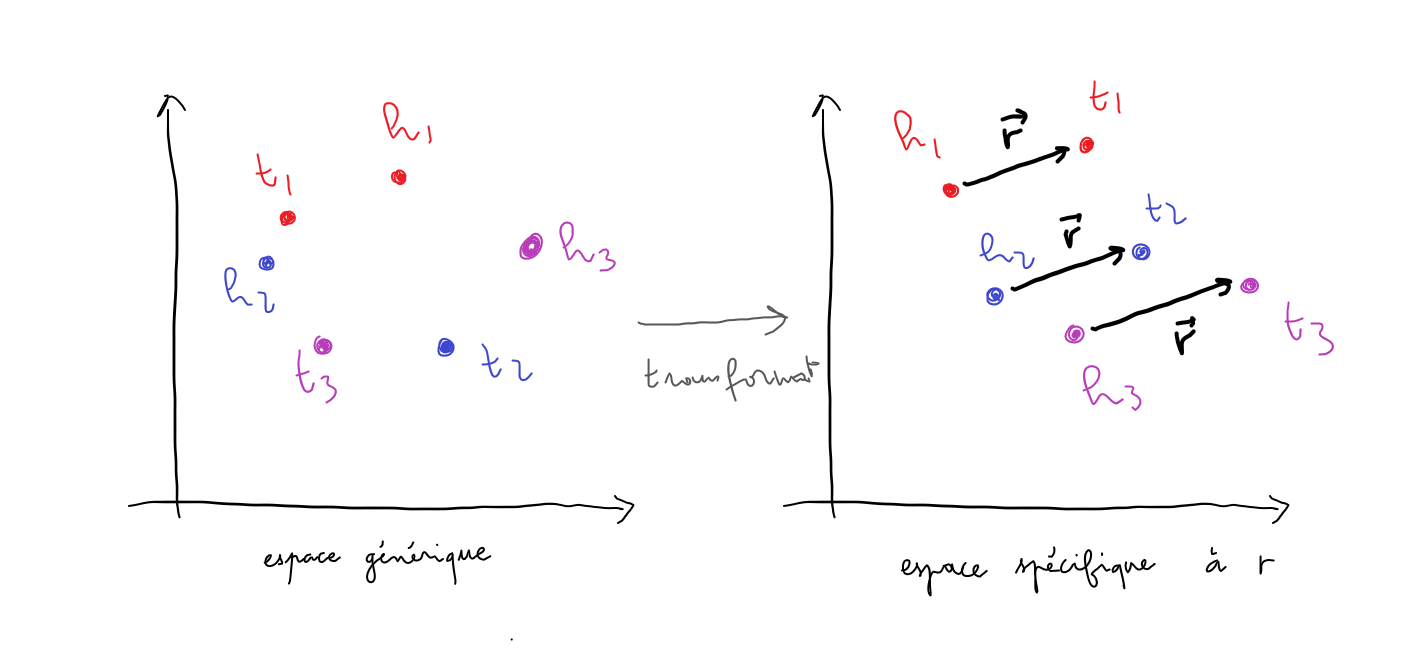
\includegraphics[width=\textwidth]{img/transd_schema.png}
    \begin{tikzpicture}[
  arrow/.style={->, shorten >=3pt, gray!80},
  point/.style={circle,inner sep=0, minimum height=0.2cm, draw=#1, fill=#1, node distance=0.1cm},
]

\def\X{5}
\def\Y{5}
\begin{scope}
    \node (o) at (0, 0) {};
    \node (ax) at (\X, 0) {};
    \node (ay) at (0, \Y) {};
    \draw[axis] (o.center) to (ax);
    \draw[axis] (o.center) to (ay);
    
    \node[point=accent1, label={[accent1]$h_1$}] (h1) at (0.5*\X, 0.8*\Y) {};
    \node[point=accent1, label={[accent1]$t_1$}] (t1) at (0.2*\X, 0.7*\Y) {}; 
    \node[point=accent2, label={[accent2]$h_2$}] (h2) at (0.15*\X, 0.55*\Y) {};
    \node[point=accent2, label={[accent2]$t_2$}] (t2) at (0.45*\X, 0.45*\Y) {}; 
    \node[point=purple, label={[purple]$h_3$}] (h3) at (0.25*\X, 0.3*\Y) {};
    \node[point=purple, label={[purple]$t_3$}] (t3) at (0.65*\X, 0.65*\Y) {}; 
    \node at (0.5*\X, -0.5) {Espace générique};
    
    \draw[->, accent1, thick] (\X, 0.5*\Y) to node[above, red] {transformation}  (\X+3, 0.5*\Y);
\end{scope}

\begin{scope}[xshift=8.5cm]
    \node (o) at (0, 0) {};
    \node (ax) at (\X, 0) {};
    \node (ay) at (0, \Y) {};
    \draw[axis] (o.center) to (ax);
    \draw[axis] (o.center) to (ay);
    
    \def\dx{3}
    \def\dy{0.7}
    
    \node[point=accent1, label={[accent1]$h_1$}] (h1) at (0.5*\X, 0.8*\Y) {};
    \node[point=accent1, label={[accent1]$t_1$}, above right=\dy and \dx of h1] (t1) {}; 
    \node[point=accent2, label={[accent2]$h_2$}] (h2) at (0.15*\X, 0.55*\Y) {};
    \node[point=accent2, label={[accent2]$t_2$}, above right=\dy and \dx of h2] (t2) {}; 
    \node[point=purple, label={[purple]$h_3$}] (h3) at (0.25*\X, 0.3*\Y) {};
    \node[point=purple, label={[purple]$t_3$}, above right=\dy and \dx of h3] (t3)  {}; 
    
    \draw[vec] (h1) to node[sloped, above] {$\vec{r}$} (t1);
    \draw[vec] (h2) to node[sloped, above] {$\vec{r}$} (t2);
    \draw[vec] (h3) to node[sloped, above] {$\vec{r}$} (t3);
    \node at (0.5*\X, -0.5) {Espace spécifique à $r$};
\end{scope}
\end{tikzpicture}
    \caption[Principe du modèle TransD]{Représentation du modèle TransD, avec à gauche l'espace des plongements $\bf{e}$, et à droite l'espace des plongements transformés $M_{e, r} \cdot \bf{e}$ (tiré de \cite{transd}).}
    \label{fig:transd-schema}
\end{figure}

Soit finalement une fonction d'énergie :
\begin{equation}
    E_\Theta(h, r, t) = \| (\bf{r_p \cdot h_p^\top + I_{d' \times d}}) \cdot \bf{h} + \mathbf{r} - (\bf{r_p \cdot t_p^\top + I_{d' \times d}}) \cdot \bf{t} \|_2 
\end{equation}
À nouveau, cette équation se ré-écrit comme l'équation de TransE avec un terme correcteur $\bf{r_p} \cdot (\bf{ h_p^\top \cdot h - t_p^\top \cdot t})$:
\begin{equation}
    E_\Theta(h, r, t) = \| (\bf{h + r - t}) + \bf{r_p} \cdot (\bf{ h_p^\top \cdot h - t_p^\top \cdot t}) \|_2 
\end{equation}



\begin{table}[ht]
\caption{Propriétés de quelques modèles à translation}
\centering
\begin{tabular}{|c|c|c|c|c|}
\hline %\rowcolor[gray]{0.8}\color{black}
Modèle & Entités & Relations & Transformation & Nombre de paramètres\\\hline
TransE & $\mathbf{e} \in \mathbb{R}^d$ & $\mathbf{r} \in \mathbb{R}^d$ & Aucune & $d \times (m + n)$ \\
TransH & $\mathbf{e} \in \mathbb{R}^d$ & $\mathbf{r, n_r} \in \mathbb{R}^d$ & Projection sur un hyperplan & $d \times (2m + n)$ \\
TransD & $\mathbf{e, e_p} \in \mathbb{R}^d$ & $\mathbf{r, r_p} \in \mathbb{R}^d$  & Transformation linéaire & $2d \times (m + n)$ \\\hline
\end{tabular}
\label{tab:transx}
\end{table}

\FloatBarrier

\subsection{Autres modèles}
\label{subsec:kge-models-misc}

\subsubsection{RDF2Vec}

Le modèle RDF2Vec s'inspire du modèle de plongement Word2Vec \cite{mikolov2013distributed}, très utilisé pour produire des plongements lexicaux.

Il fonctionne en deux étapes. % : d'abord, des chemins sont prélevés dans le graphe de connaissance au moyen de marches aléatoires – ces chemins sont simplement des suites d'entités et de relations connectées entre elles. % Pour les prélever, on commence par tirer aléatoirement une entité 
Dans un premier temps, des chemins sont prélevés dans le graphe au moyen de marches aléatoires.
Un \textit{chemin} sur le graphe est une suite d'entités et de relations $(x_1, x_2, \ldots, x_T)$ tels que, pour tout $k \in \{1, 2, \ldots, \frac{T}{2}\}$, $x_{2k-1}$ est une entité, $x_{2k}$ est une relation, et $(x_{2k-1}, x_{2k}, x_{2k+1})$ est un triplet valide de $\KG$. Par exemple, la séquence \texttt{(dbr:Picasso, dbo:birthPlace, dbr:Málaga, dbo:country, dbr:Spain)} est un chemin de longueur 5, constitué des triplets \texttt{(dbr:Picasso, dbo:birthPlace, dbr:Málaga)} et \texttt{(dbr:Málaga, \allowbreak dbo:country, dbr:Spain)}. 
Dans un tel chemin, le \textit{contexte} d'un élément $x_i$ est l'ensemble des $c$ éléments précédant $x_i$ et des $c$ éléments le suivant, avec $c$ un paramètre appelé la \textit{longueur}
du contexte. On le note :
 \begin{equation}
    x_{t \pm c} = (x_{t-c}, x_{t-c+1}, \ldots, x_{t-1}, x_{t+1}, \ldots, x_{t+c})
\end{equation}
 Pour chaque entité $e$ du graphe, on effectue des marches aléatoires de longueur $T$ au départ de $e$ pour former un ensemble de séquences $S_e$ : il suffit pour cela d'effectuer une recherche en profondeur à partir de $e$, et de s'arrêter lorqu'on atteint une profondeur $T$. Ces marches aléatoires constituent le jeu d'entraînement.

% Ajouter l'équation pour définir une marche aléatoire

Ensuite, ces chemins sont passés en entrée à un réseau de neurones. Deux variantes existents : dans la version C-BoW, le but de ce réseau est de prédire une entité en fonction des plongements de son contexte; dans la version Skip-Gram, il s'agit au contraire de prédire le contexte d'une entité à partir du plongement de celle-ci.

\paragraph{C-BoW}

Dans cette variante, le réseau de neurones prend en entrée le contexte  $x_{t \pm c}$ d'un élément; son objectif est de prédire l'élément cible $x_t$ à partir de ce contexte.

%Dans cette variante, le réseau de neurone prend en entrée une partie d'un chemin, constituée des $c$ éléments précédant l'élément $x_t$ et des $c$ éléments le suivant. La longueur du contexte $c$ est un paramètre; ces $2c$ éléments sont appelés le \textit{contexte} de $x_t$ et sont notés :
%\begin{equation}
%    x_{t \pm c} = (x_{t-c}, x_{t-c+1}, \ldots, x_{t-1}, x_{t+1}, \ldots, x_{t+c})
%\end{equation}
%L'objectif du modèle est de prédire l'élément cible $x_t$ à partir de son contexte $x_{t \pm c}$.

Tout élément $x \in \Ent \cup \Rel$ possède un plongement vectoriel $\bf{x}$ dans $\R^d$, obtenu par une couche de projection. Le contexte $x_{t \pm c}$ est représenté comme la moyenne des plongements de ses éléments :
\begin{equation}
    \compconj{\bf{x}_t} = \frac{1}{2c} \sum_{-c \leq i \leq c, i \neq t} \bf{x}_{t+i}
\end{equation}

Le modèle attribue une probabilité que $x_t$ soit effectivement égal à $x$, définie comme un softmax sur tout le vocabulaire $\Ent \cup \Rel$ :
\begin{equation}
    P(x | x_{t \pm c}) = \frac{\displaystyle \exp(\compconj{\bf{x}_t}^\top \bf{x})}{\displaystyle \sum_{y \in \Ent \cup \Rel} \exp(\compconj{\bf{x}_t}^\top \bf{y})}
\end{equation}

Enfin, on fait glisser la fenêtre de contexte sur toute longueur de la séquence d'entraînement; l'objectif du modèle est alors de maximiser la log-probabilité de la séquence complète :
\begin{equation}
    \frac{1}{T} \sum_{t = 1}^{T} \log P(x_t | x_{t \pm c})
\end{equation}

Cette architecture est représentée à la figure \ref{fig:rdf2vec-cbow}. En entrée, les éléments sont représentés par des vecteurs \textit{one-hot} : si on note $(w_1, w_2, \ldots, w_V)$ les éléments de $\Ent \cup \Rel$, avec $V = | \Ent \cup \Rel |$, alors le vecteur \textit{one-hot} de l'élément $w_i$ est un vecteur de dimension $V$ contenant des zéros et un unique $1$ à la $i$-ème coordonnée.

\begin{figure}[h]
    \centering
    \begin{tikzpicture} [
            neuron/.style={fill=gray!20, draw=gray!40, circle},
            rel/.style={fill=gray!40, ->}
        ]
\def\offsety{0.75}
\def\offsetx{1}

\def\ypos{-1.5}
\node[label={180:\textit{Entrée}}] at (0*\offsetx, \ypos*\offsety) {};
\node at (2*\offsetx, \ypos*\offsety) {\textit{Projection}};
\node[label={0:\textit{Sortie}}] at (4*\offsetx, \ypos*\offsety) {};

\node [neuron, label={180:\texttt{Picasso}}] (0) at (0, 3*\offsety) {};
\node [neuron, label={180:\texttt{dbo:birthPlace}}] (1) at (0, 2*\offsety) {};
\node [neuron, label={180:\texttt{dbo:country}}] (2) at (0, 1*\offsety) {};
\node [neuron, label={180:\texttt{Spain}}] (3) at (0, 0*\offsety) {};
\node [neuron] (4) at (2, 1.5*\offsety) {$\Sigma$};
\node [neuron, label={0:\texttt{Málaga}}] (5) at (4, 1.5*\offsety) {};

\draw [style=rel] (0) to (4);
\draw [style=rel] (1) to (4);
\draw [style=rel] (2) to (4);
\draw [style=rel] (3) to (4);
\draw [style=rel] (4) to (5);
        
\end{tikzpicture}
    \caption[Architecture de RDF2Vec-CBoW]{L'architecture du modèle RDF2Vec dans sa variante C-BoW.}
    \label{fig:rdf2vec-cbow}
\end{figure}

\paragraph{Skip-Gram}

Skip-Gram opère à l'inverse de C-BoW : l'objectif est ici de prédire le contexte à partir de l'élément cible. On dispose à nouveau d'un élément cible $x_t$ et de son contexte; le modèle projette $x_t$ dans $\R^d$ avec une couche de projection. Le modèle attribue alors à tout élément $x$ du vocabulaire $\Ent \cup \Rel$ une probabilité : la probabilité que $x$ fasse partie du contexte de $x_t$. Cette probabilité s'exprime :
\begin{equation}
    P(x | x_t) = \frac{
    \displaystyle \exp(\bf{x}^\top \bf{x}_t)}
    {\displaystyle \sum_{y \in \Ent \cup \Rel} \exp(\bf{y}^\top \bf{x}_t)}
\end{equation}

On moyenne alors cette probabilité pour tous les éléments du contexte, pour chaque élément cible de la séquence, ce qui donne la log-probabilité moyenne du contexte, qui doit être maximisée par le modèle :
\begin{equation}
    \frac{1}{T} \sum_{t = 1}^{T} \sum_{-c \leq i \leq c, i \neq t} \log P(x_{t+i} \mid x_t)
\end{equation}

Cette architecture est présentée à la figure \ref{fig:rdf2vec-skipgram}; comme précédemment, l'élément d'entrée est représenté par son vecteur \textit{one-hot}.

\begin{figure}[h]
    \centering
    \begin{tikzpicture} [
            neuron/.style={fill=gray!20, draw=gray!40, circle},
            rel/.style={fill=gray!40, <-}
        ]
\def\offsety{0.75}
\def\offsetx{-1}

\def\ypos{-1.5}
\node[label={0:\textit{Sortie}}] at (0*\offsetx, \ypos*\offsety) {};
\node at (2*\offsetx, \ypos*\offsety) {\textit{Projection}};
\node[label={180:\textit{Entrée}}] at (4*\offsetx, \ypos*\offsety) {};

\node [neuron, label={0:\texttt{Picasso}}] (0) at (0*\offsetx, 3*\offsety) {};
\node [neuron, label={0:\texttt{dbo:birthPlace}}] (1) at (0*\offsetx, 2*\offsety) {};
\node [neuron, label={0:\texttt{dbo:country}}] (2) at (0*\offsetx, 1*\offsety) {};
\node [neuron, label={0:\texttt{Spain}}] (3) at (0*\offsetx, 0*\offsety) {};
\node [neuron] (4) at (2*\offsetx, 1.5*\offsety) {$ $};
\node [neuron, label={180:\texttt{Málaga}}] (5) at (4*\offsetx, 1.5*\offsety) {};

\draw [style=rel] (0) to (4);
\draw [style=rel] (1) to (4);
\draw [style=rel] (2) to (4);
\draw [style=rel] (3) to (4);
\draw [style=rel] (4) to (5);
        
\end{tikzpicture}
    \caption[Architecture de RDF2Vec-Skip-Gram]{L'architecture du modèle RDF2Vec dans sa variante Skip-Gram.}
    \label{fig:rdf2vec-skipgram}
\end{figure}

À la fin de l'entraînement, il suffit de récupérer les poids de la couche cachée pour obtenir les plongements vectoriels des entités et des relations.

 


\FloatBarrier


\section{Séparabilité des plongements vectoriels}
Puisque le but général de ce travail est d'identifier des groupes sémantiquement cohérents d'entités à partir de leur proximité géométrique, il nous est nécessaire d'évaluer la capacité d'un modèle à plonger les instances d'une même classe dans la même région de l'espace euclidien. On formalise cette exigence en définissant une tâche de séparabilité, dont le but est de mesurer si des groupes d'entités appartenant à deux classes différentes sont linéairement séparables.

Le principe général est le suivant : pour deux classes $A$ et $B$, on prélève aléatoirement $N$ instances de $A$ et $N$ instances de $B$; on attribue aux instances de $A$ l'étiquette $0$ et à celles de $B$ l'étiquette $1$. Le résultat est un jeu de données $D = \{\mathbf{e_i}, y_i \}_{i=1, \ldots, 2N}$, avec $\bf{e}_i \in \R^d$ le plongement vectoriel de l'entité $e_i$, et $y_i \in \{ 0, 1\}$ l'étiquette associée à $e_i$. On entraîne alors une SVM linéaire sur 75\% de ces points, et on prédit ensuite les étiquettes des 25\% restant. Les étiquettes prédites peuvent alors êtres prédites aux étiquettes d'origine, selon les mesures usueles de la classification automatique : précision, rappel, mesure $F1$. Dans nos expériences, on choisit $N=1000$; si une classe possède moins que ces $N$ instances, on utilise toutes les instances de cette classe.

\subsubsection{Variables d'analyse}

La difficulté qu'il y a à séparer une classe $A$ d'une classe $B$ dépends beaucoup de $A$ et de $B$ : intuitivement, il est plus difficile de distinguer un \dbo{College} d'une \dbo{University} qu'un \dbo{Aircraft} d'une \dbo{Person}. De plus, on peut imaginer que la taille de la classe (c'est-à-dire le nombre d'instances qui en font partie) influe aussi sur la difficulté, comme c'est souvent le cas en apprentissage automatique. Nous avons donc mis au point trois métriques pour évaluer la difficulté \textit{a priori} de la tâche de séparation pour toute paire de classe $(A, B)$. La première de ces métriques est la distance lexicale entre les classes, mesurée grâce à des plongements lexicaux; la deuxième est une distance taxonomique entre les classes, basée sur la distance entre les classes dans l'arbre; la troisième est un indicateur de la fréquence des deux classes dans la base de connaissance.

Ces métriques permettent d'interpréter les résultats de séparabilité obtenus et d'identifier les modèles qui parviennent le mieux à séparer les classes proches ou les classes rares. On les détaille dans les trois paragraphes suivants.


\paragraph{Distance lexicale}

La première de nos métriques est une distance entre les classes, basée sur la proximité sémantique des noms de ces classes. Pour une classe $X$ quelconque, on commence par séparer les mots qui composent son URI : dans DBpédia, la convention de nommage pour les classes est le \textit{CamelCase}, donc l'entité \texttt{SportsTeamMember} est séparée en \texttt{"sports"}, \texttt{"team"} et \texttt{"member"}. On utilise alors des plongements lexicaux pour représenter chacun de ces mots par un vecteur de $\R^d$, et on moyenne ensuite ces vecteurs pour obtenir une représentation vectorielle $\mathbf{X}$ de la classe $X$ de départ. On peut alors définir la distance entre deux classes $A$ et $B$ comme la distance euclidienne entre leurs représentants :
\begin{equation}
d_\text{lex}(A, B) = \| \mathbf{A} - \mathbf{B} \|_2
\end{equation}

Les plongements lexicaux utilisés sont entraînés avec CBOW \cite{mikolov2018advances} sur le Common Crawl, un corpus en anglais comprenant 600 milliards de mots et deux millions de types distincts.

%\footnote{We used word embeddings from \href{https://fasttext.cc/docs/en/english-vectors.html}{https://fasttext.cc/docs/en/english-vectors.html}, trained on Common Crawl \cite{mikolov2018advances}} 

\paragraph{Distance taxonomique}
On introduit également une distance entre les classes basée sur leur distance dans la taxonomie de départ. Puisqu'une taxonomie est un arbre, il existe un unique chemin (non-orienté) de longueur minimale entre n'importe quelle paire de classes $A$ et $B$ dans la taxonomie. En effet, un arbre est un graphe connexe minimal : connexe, donc au moins un chemin existe entre $A$ et $B$; minimal, donc il ne peut exister qu'un chemin, sinon on pourrait supprimer une arête d'un des deux chemins sans perdre la connexité, ce qui contredirait la minimalité du graphe. On note donc $\text{path}(A, B) = \{(A \rightarrow c_1), (c_1 \rightarrow c_2), \ldots, (c_k \rightarrow B)\}$ ce chemin. Pour une arête $e = (c_i \rightarrow c_j)$ donnée, on définit également sa profondeur $\text{depth}(e)$ comme le nombre d'arêtes entre elle et la racine de l'arbre : une arête connectée directement à la racine a une profondeur nulle; une arête connectée à un successeur immédiat de la racine a une profondeur égale à $1$, etc.
On peut alors définir la distance taxonomique comme :
\begin{equation}
    d_\text{tax}(A, B) = \sum_{e \in \text{path}(A, B)} \frac{1}{\displaystyle 2^{\text{depth}(e)}}
\end{equation}
Cette distance taxonomique est la longueur du chemin entre $A$ et $B$, pondérée par la profondeur des arêtes qui composent ce chemin. Le poids d'une arête est $1/2^{\text{depth}(e)}$ et diminue donc avec sa profondeur : en effet, dans une taxonomie, la profondeur d'une arête est un indicateur de la spécificité de l'axiome de subsumption associé à cette arête. Les axiomes associés aux arêtes de profondeur $0$ sont des axiomes très généraux, comme par exemple $\dbo{Place} \sqsubseteq \texttt{owl:Thing}$ («un endroit est une chose») ou $\dbo{Agent} \sqsubseteq \texttt{owl:Thing}$ («un agent est une chose»). À la profondeur $1$, les axiomes sont déjà plus précis – par exemple, $\dbo{Person}\sqsubseteq \dbo{Agent}$ («une personne est un agent»). À des profondeurs plus élevés, les axiomes deviennent très spécifiques, comme par exemple $\dbo{MotorRace} \sqsubseteq \dbo{Race}$ à la profondeur $4$. Aussi, deux classes séparées par une arête de faible profondeur sont plus sémantiquement plus distantes que deux classes séparées par une arête de profondeur élevée.

Quant au choix d'une décroissance spécifiquement égale à $\frac{1}{2^k}$, il confère à notre distance une propriété intéressante : une classe $A$ est plus proche de ses sous-classes que de n'importe quelle autre classe. Vérifions-le en prenant $A$ une classe de profondeur $d$, et $A'$ une sous-classe de $A$ de profondeur $d' > d$. Alors la distance entre $A$ et $A'$ s'écrit :
\begin{align*}
    d_\text{tax}(A, A') &= \sum_{k = d}^{d'-1} 2^{-k} \\
    &= 2^{-d} \cdot \sum_{k=0}^{d'-d-1} 2^{-k} \\
    &= \frac{1}{2^{d-1}} \left(1 - \frac{1}{2^{d'-d}} \right) 
\end{align*}
Or la distance entre $A$ et sa superclasse immédiate $B$ est :
\begin{align*}
    d_\text{tax}(A, B) &= \frac{1}{2^{d-1}} \\
\end{align*}
Et $d'-d \geq 1$, donc $d_\text{tax}(A, A') < \frac{1}{2^{d-1}} = d_\text{tax}(A, B) \leq d_\text{tax}(A, B')$ pour toute classe $B'$ qui n'est pas sous-classe de $A$. On retrouve bien la propriété énoncée.

\paragraph{Influence de la fréquence}

Une entité $e$ impliquée dans de nombreux triplets sera vue plus souvent pendant la phase d'entraînement, et aura donc un plongement vectoriel plus fiable. Comme ce plongement vectoriel dépend à son tour des plongements des entités et des relations qui sont connectée à $e$, il est possible que les entités appartenant à des classes rares soient impliqués dans des relations rares elles-aussi et connectées à des entités rares; cela produirait des plongements vectoriels moins fiable que la moyenne. Pour vérifier cette hypothèse, on évalue également l'influence de l'effectif des classes (\textit{i.e.} le nombre d'instances qui appartiennent à cette classe) sur les scores de séparabilité. Pour obtenir une mesure synthétique de la fréquence d'une paire de classe $(A, B)$, on utilise la moyenne harmonique des fréquences de $A$ et de $B$. L'utilisation de la moyenne harmonique plutôt que de la moyenne arithmétique usuelle permet de mieux refléter les déséquilibres entre les fréquences de $A$ et de $B$ : si $N_A$ est la fréquence de la classe $A$ et $N_B$ celle de la classe $B$, et que $N_A$ est supérieur à $N_B$ d'un ordre de grandeur, alors la moyenne arithmétique de $N_A$ et $N_B$ a le même ordre de grandeur que $N_A$, et n'indique donc pas que $B$ est rare par rapport à $A$.

\subsection{Résultats}

On évalue six modèles de plongement sur la tâche de séparabilité : TransE, TransH, TransD, DistMult, ComplEx, RDF2Vec. La séparabilité est calculée sur 10 000 paires de classes issues de DBpédia. On donne les scores de séparabilité moyens pour chaque modèle dans le tableau \ref{tab:separability-results}; on aggrège également les résultats pour différentes valeurs de distance lexicale et taxonomique dans la figure \ref{fig:separability-lexical}, et pour différentes fréquences de classes dans la figure \ref{fig:separability-freq}.


\begin{table}[]
    \centering
    \caption{Précision, rappel et mesure $F1$ moyens pour différents modèles de plongement sur la tâche de séparabilité. En gras, le meilleur résultat pour chaque métrique.}
    \begin{tabular}{|lrrr|}
    \hline 
        Modèle     & Précision  & Rappel & $F1$ \\
        \hline 
        ComplEx   &	90.4	&	89.9	&	89.7 \\
        DistMult  &	92.5	&	91.6	&	91.6 \\
        RDF2Vec   &	\textbf{99.7}	&	\textbf{99.7}	&	\textbf{99.7} \\
        TransE    &	99.4	&	99.1	&	99.2 \\
        TransH    &	93.6	&	92.1	&	92.5 \\
        TransD    &	85.0	&	83.1	&	83.5 \\
        \hline
    \end{tabular}
    \label{tab:separability-results}
\end{table}

\begin{figure}[h]
  \centering
  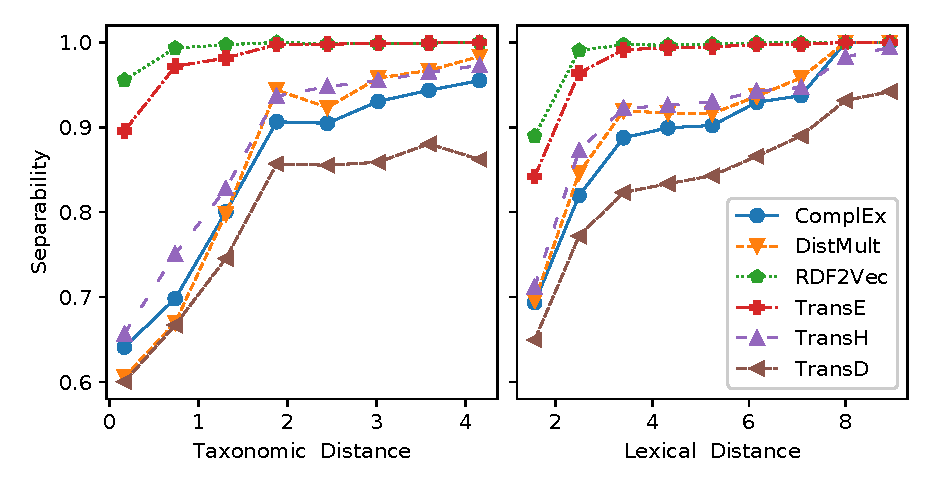
\includegraphics[width=0.8\textwidth]{fig/plot/sep1_dist.eps}
  \caption{Séparabilité moyenne entre deux classes en fonction de leur distance taxonomique (à gauche) et de leur distance lexicale (à droite), pour différents modèles de plongement. }
  \label{fig:separability-lexical}
\end{figure}

\begin{figure}[h]
  \centering
  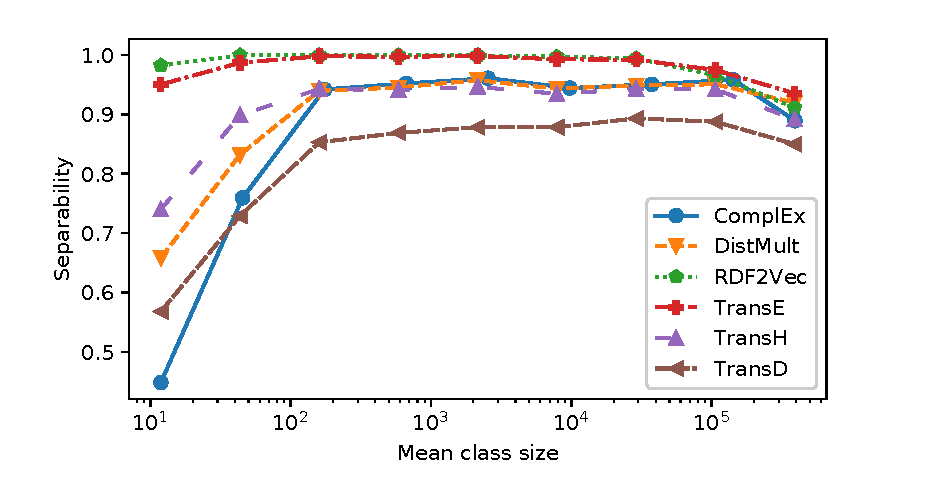
\includegraphics[width=0.8\linewidth]{fig/plot/separability2_type1.eps}
  \caption{Séparabilité moyenne entre deux classes en fonction de la fréquence de ces classes, pour différents modèles de plongement.}
  \label{fig:separability-freq}
\end{figure}

Comme attendu, le score de séparabilité est dépendant de la distance lexicale et taxonomique entre les classes, et ce pour tous les modèles. Tous les modèles sauf TransD parviennent à séparer correctement les classes distantes (distance lexicale supérieur à 8, ou distance taxonomique supérieure à 3); en revanche, seuls deux modèles parviennent à conserver des scores élevés sur l'essentiel de l'intervalle : RDF2Vec et TransE, avec un avantage net pour RDF2Vec dans les faibles distances. La séparabilité moyenne de ces deux modèles diminue pour les classes très proches (distance taxonomique inférieure à 1, distance lexicale inférieure à 2), mais elle demeure supérieure à 85\%. Tous les autres modèles obtiennent des résultats nettement inférieurs.

Dans la figure \ref{fig:separability-freq}, on observe que les classes rares sont plus difficilement séparables que les classes fréquentes, quoique tous les modèles n'ont pas la même sensibilité à la fréquence : RDF2Vec et TransE n'ont qu'une légère baisse de score pour les classes rares (moins de $10^2$ instances en moyenne), qui peut partiellement être causée par le faible nombre d'échantillons sur lesquels entraîner la SVM. En revanche, les autres modèles ComplEx, DistMult, TransH et TransD y sont très sensibles. Cette sensibilité ne s'explique pas par une corrélation entre les paires rares et les paires proches, puisque les coefficients de Spearman et de Pearson entre les variables de distance et de fréquence sont proches de zéro.

%we observe that rare classes are indeed less separable than more frequent classes, with some variability depending on embedding models. RDF2Vec is once again the best model, with TransE slightly behind. TransH, DistMult and ComplEx have close scores in the size range $[200, 10^5]$, but ComplEx is more sensitive to rare classes than DistMult, which is itself more sensitive than TransH. More surprisingly, we observe that scores also decrease for very frequent classes (mean size above $10^5$ instances) for all embedding models. Both Pearson and Spearman’s correlations between lexical distance and mean class size are close to zero, which rules out the possibility of a bias in the dataset. An explanation is that frequent classes are more likely to be parent of other classes in the dataset (for example, \texttt{dbo:Agent} is the second most frequent class of the dataset, and is a parent of half the classes in the DBpedia ontology), and separating a subclass from its parent is harder than separating sibling or unrelated classes. Finally, we observe a convergence of scores for frequent classes between all models, with TransE achieving the highest score.

En résumé, seuls deux modèles obtiennent une mesure $F1$ moyenne supérieure à 95\% sur notre tâche de séparabilité : RDF2Vec et TransE, avec respectivement 99,7\% et 99,2\% respectivement. 
%\label{sec:kge-sep}

